\documentclass[12pt, letterpaper]{article}
\usepackage{graphicx} % Required for inserting images
\usepackage{hyperref}
\usepackage{xcolor}
\usepackage{amssymb}
\usepackage{amsmath}
\usepackage[english]{babel}
\usepackage{nicefrac, xfrac}
\usepackage{tikz}
\newcommand{\Z}{{\mathbb Z}}
\newcommand{\R}{{\mathbb R}}
\newcommand{\N}{{\mathbb N}}
\newcommand{\dimo}{{\text{\textbf{Dimostrazione }:}}}
\newcommand{\mcm}{{\text{mcm}}}
\newcommand{\MCD}{{\text{MCD}}}
\newcommand{\aut}{{\text{Aut}}}
\newcommand{\cen}{{\text{Centro}}}
\newcommand{\norm}{{\unlhd}}
\newcommand{\ciclS}{{\left \langle }}
\newcommand{\ciclE}{{\right \rangle }}
\usetikzlibrary{positioning}
\usepackage[paper=a4paper,left=20mm,right=20mm,bottom=25mm,top=25mm]{geometry}
\title{Algebra}
\author{Marco Casu}
\date{\vspace{-5ex}}
\begin{document}
\newcommand{\omo}[1]{\(\varphi\)}


\maketitle
\begin{figure}[h]
    \centering{
    
\includegraphics[width=0.8\textwidth ]{images/Copertina2.png}
    }
\end{figure}
\newpage 
\tableofcontents
\newpage
\section{Insiemi e Relazioni}
Sappiamo già che un insieme non è altro di una collezione di oggetti distinti.\raggedright\\
\centering
\(A=\{1,2,3,4,5\}\)\\
\raggedright
Ricapitoliamo le proprietà basiche degli insiemi : 
\begin{itemize}
    \item \textbf{Intersezione} - \(A \cap B \rightarrow \{x | x\in A \land x\in B\}\)
    \item \textbf{Unione} - \(A \cup B \rightarrow \{x | x\in A \lor x\in B\}\)  
    \item \textbf{Sottoinsieme} - \(A \subseteq B \rightarrow  \{x\in A \implies x \in B\}\)
    \item \textbf{Insieme complementare} - \(A^c_{\text{in B}} \rightarrow \{x\in B | x \notin A\}\)
\end{itemize}
\subsection{Proprietà fondamentali degli insiemi}
Elenchiamo le già note proprietà degli insiemi :
\begin{itemize}
    \item \textbf{Associativa} - \( (A \cap B)\cap C =  (C \cap B)\cap A \)  oppure   \( (A \cup B)\cup C =  (C \cup B)\cup A \)
    \item \textbf{De Morgan} - Se \(A, B \subseteq C\) allora \((A \cap B)^c = A^c \cup B^c\) oppure \((A \cup B)^c = A^c \cap B^c\) 
    \item \textbf{Distributiva} - \( (A\cup B)\cap C = (A \cap C)\cup(B \cap C)  \) oppure \( (A\cap B)\cup C = (A \cup C)\cap(B \cup C)  \)
\end{itemize}
Un insieme particolare associato ad un dato insieme \(A\) è \textbf{l'insieme delle parti} di \(A\),
è l'insieme di tutti i possibili sotto-insiemi di \(A\) e si indica con :
\begin{equation}
    \mathcal{P}(A) = \{ B | B \subseteq A \}
\end{equation}
\\Introduciamo adesso il concetto di \textbf{prodotto cartesiano} su due insiemi \(A\) e \(B\),
 esso non è altro che l'insieme di tutte le coppie ordinate dove il primo elemento appartiene ad \(A\)
 ed il secondo elemento a \(B\) :
 \begin{equation}
    A \times B = \{ (a,b) | a\in A, b\in B\}
 \end{equation}
\subsection{Le Relazioni}
Una relazione \(\rho\) da un insieme \(A\) ad un insieme \(B\), è un sotto-insieme del prodotto
cartesiano \( A \times B\).
\begin{equation}
    \rho \subseteq A \times B \text{,  se } (a,b)\in \rho \text{ si scrive }a\rho b
\end{equation}
Il dominio di tale relazione \(\rho\) risulta essere :
\begin{equation}
    \mathcal{D}(\rho)=\{a\in A | \exists b\in B \text{ per il quale risulti }a\rho b\}
\end{equation}
La sua immagine : 
\begin{equation}
    \Im(\rho)=\{b\in B | \exists a\in A \text{ per il quale risulti }a\rho b\}
\end{equation}
Per una relazione \(\rho\), se il suo dominio risulta essere tutto \(A\), e 
\(\forall a\in A \exists \text{ un unico } b \in B | a\rho b\), tale \(\rho\) è 
anche una \textbf{funzione}.
\\\textit{Esempio di relazione : }\\
sia \(A=\{a,b,c,d\}\), è definita la relazione \(\rho \subseteq A\times A = \{(a,b),(b,c),(c,c),(c,a),(d,b)\}\).
\newpage Abbiamo due modi per poter visualizzare una relazione, un formato tabellare, ed un formato 
con nodi e collegamenti fra gli elementi della relazione. Per la relazione \(\rho \) appena enunciata si ha la seguente rappresentazione tabellare
dove si inserisce un 1 nel punto in cui le due coordinate sono in relazione fra loro : 
\\ \hphantom{.}\\
\centering
\begin{tabular}{ c c c c c }
    \(d\) & 0 & 0 & 0 & 0  \\ 
    \(c\) & 0 & 1 & 1 & 0  \\ 
    \(b\) & 1 & 0 & 0 & 1  \\ 
    \(a\) & 0 & 0 & 1 & 0  \\ 
    &\(a\) & \(b\) & \(c\) & \(d\) 
        
   \end{tabular}
\\ 
 \hphantom{.}\\
 \raggedright
Vediamone adesso una rappresentazione con nodi e collegamenti : 
 \\
 \centering
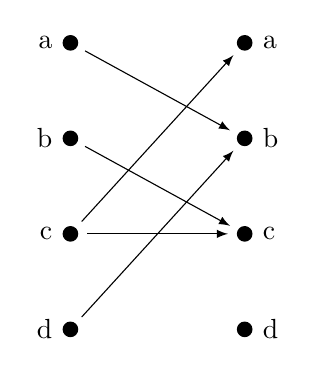
\begin{tikzpicture}[
    mydot/.style={
      circle,
      fill,
      inner sep=2pt
    },
    >=latex,
    shorten >= 3pt,
    shorten <= 3pt
    ]
    \node[mydot,label={left:a}] (a1) {}; 
    \node[mydot,below=of a1,label={left:b}] (a2) {}; 
    \node[mydot,below=of a2,label={left:c}] (a3) {}; 
    \node[mydot,below=of a3,label={left:d}] (a4) {}; 
    
    \node[mydot,right=2cm of a1,label={right:a}] (b1) {}; 
    \node[mydot,below=of b1,label={right:b}] (b2) {}; 
    \node[mydot,below=of b2,label={right:c}] (b3) {}; 
    \node[mydot,below=of b3,label={right:d}] (b4) {}; 
    
    \path[->] (a1) edge (b2);
    \path[->] (a2) edge (b3);
    \path[->] (a3) edge (b1)
      edge (b3);
    \path[->] (a4) edge (b2) ;
    
    \end{tikzpicture}
    \\ 
 \raggedright
 Essendo le relazioni degli insiemi, possiamo considerare le operazioni di unione ed intersezione
 anche per le relazioni. Esista per ogni relazione, anche la sua \textbf{relazione inversa},
 se \(\rho\) è definita da \(A\) a \(B\), esisterà \(\rho^{-1}\) definita da \(B\) a \(A\).
 \begin{equation}
    \rho^{-1} = \{ (b,a) \in B\times A | a\rho b\} \text{ quindi } a\rho b \implies b\rho^{-1} a
 \end{equation}
 Se la relazione \(\rho\) è una funzione, non è detto che la sua relazione inversa sia una funzione anch'essa,
 prendiamo ad esempio la relazione \(\rho \subset \mathbb{R} \times \mathbb{R}  =\{ (x,x^2) \forall a\in \mathbb{R}\}\), che non è altro che
 la funzione di una variabile reale \(f(x)=x^2\). Tale funzione, per \(x=-a\) ed \(x=a\), ha sempre \(f(x)=a^2\), per due valori
 appartenti al dominio ha la stessa immagine, la sua funzione inversa avrebbe quindi un punto che mappa due immagini.
\\\hphantom{.}\\
Una relazione nota su insieme \(A\) è la \textbf{relazione identità}, definita : \(\Delta_A = \{(a,a)\in A \times A\}\).
\subsection{Relazioni di Equivalenza}
Una relazione \(\rho\) definita su un insieme \(A\), quindi \(\rho \subseteq A \times A\), è detta \textbf{relazione 
di equivalenza} se soddisfa i seguenti requisiti : 
\begin{itemize}
    \item \(\rho\) è \textbf{riflessiva}, ossia è vero che :  \(a\rho a \forall a \in A\)
    \item \(\rho\) è \textbf{simmetrica}, ossia è vero che se esiste \(a\rho a'\) allora esiste \(a'\rho a\)
    \item \(\rho\) è \textbf{transitiva}, se esistono \(a\rho a'\) e \(a'\rho a''\), allora esiste \(a\rho a''\)
\end{itemize}
Un esempio di relazione di equivalenza è la relazione di \textit{avere la stessa età} su un 
insieme di studenti, difatti soddisfa tutti e 3 i requisiti : 
\begin{itemize}
    \item è \textbf{riflessiva} perchè ognuno ha la stessa età di se stesso.
    \item è \textbf{simmetrica} perchè se tizio ha la stessa età di caio, caio ha la stessa età di tizio.
    \item è \textbf{transitiva} perchè se tizio ha la stessa età di caio e caio ha la stessa età di sempronio, tizio ha la stessa età di sempronio.
\end{itemize}\newpage
Un esempio di relazione \textbf{non} di equivalenza è la relazione di \textit{genitorialità}, ad esempio non è simmetrica, perchè se 
tizio è padre di caio, caio non è assolutamente padre di tizio.
\subsection{Le Classi di Equivalenza}
Sia \(\rho\) una relazione di equivalenza definita su \(A\), si definisce \textbf{classe di equivalenza} di un 
elemento \(a\in A\), e si denota con \([a]\), l'insieme di tutti gli elementi di \(A\) che sono equivalenti (ossia in relazione di 
equivalenza) ad \(a\), ossia 
\begin{equation}
    [a] = \{b\in A | b\rho a\}
\end{equation}
Ad esempio, su una relazione di \textit{avere la stessa età}, in ogni classe di equivalenza ci sono tutte le persone
che hanno la stessa età : ogni classe può essere quindi un etichetta con il numero corrispondente all'età.
\\ \textit{Esempio esteso : }\\
Si prenda in considerazione il seguente insieme di persone :\\\centering \(A=\{\)Valentino,Marco,Luca,Alessandro,Davide\(\}\)\\
\raggedright
Ognuno ha i seguenti anni : 
\begin{itemize}
    \item Valentino - 20
    \item Marco - 19
    \item Luca - 20
    \item Alessandro - 19
    \item Davide - 19
\end{itemize}
La relazione di \textit{avere la stessa età} su \(A\) è definita come :\\ \(\rho=\{(Valentino,Luca),(Luca,Luca),(Marco,Alessandro),(Alessandro,Davide)...ecc\}\)
\\La classe di equivalenza \([Marco]=\{Marco,Alessandro,Davide\}\) definisce tutti gli elementi in relazione con \(Marco\), e rappresenta
tutte le persone di età uguale a 19.\\\hphantom{.}\\
Sia \(A\) un insieme sulla quale è definita una relazione di equivalenza, l'insieme \(\nicefrac{A}{a}\) è detto 
\textbf{insieme quoziente}, ed è l'insieme che contiene tutte le classi di equivalenza della relazione definita su \(A\).
\begin{equation}
    \nicefrac{A}{a}=\{[a], a\in A\}
\end{equation}
Vediamo adesso un \textbf{importante proprietà} delle classi di equivalenza : 
\newtheorem{theorem}{Teorema}
\begin{theorem}
\begin{equation}
    [a]=[b] \iff a\rho b
\end{equation}
\end{theorem}
\newtheorem{dimostrazione}{Dimostrazione}
\begin{dimostrazione}
    Ovviamente \(b\in [b]\) perchè \(b\rho b\), essendo  \([a]=[b] \implies b \in [a]\implies b\rho a\implies a\rho b\),
    Analogamente, se \(a\rho b\), se esiste \(c \in [a]\implies c\rho a \implies c \rho b \implies c\in [b]\implies
    [a]\subseteq[b]\).\\
    se esiste \(c \in [b]\implies c\rho b \implies c \rho a \implies c\in [a]\implies
    [b]\subseteq[a]\). Essendo \( [b]\subseteq[a]\) e \( [a]\subseteq[b]\), per forza di cose \([a]=[b]\).
\end{dimostrazione}
\raggedleft\(\blacksquare\)\newpage
\raggedright \subsubsection{Le Partizioni}
Dicesi \textbf{partizione} di un insieme \(A\) una \textit{collezione di parti o sotto-insiemi} \(A_\alpha\) non 
vuoti di \(A\) tali che \textbf{l'unione} di tutti i sotto-insiemi sia \(A\), ossia, tali collezioni \textit{ricoprono} \(A\).
\begin{equation}
    \bigcup_\alpha A_\alpha = A 
\end{equation}
Ciò significa che \(A_\alpha \cap A_\beta \ne \varnothing \implies A_\alpha = A_\beta\), in un linguaggio meno formale, tutte le partizioni 
di un insieme \(A\), non condividono nessun elemento di \(A\). Nell'immagine seguente, \(A'\) e \(A''\) sono partizioni di \(A\).
\begin{figure}[h]
    \centering{
    \includegraphics[width=0.35\textwidth ]{images/partition.eps}
    }
\end{figure}
\newtheorem{prop}{Proposizione}
\begin{prop}
    Sia \(\rho\) una relazione di equivalenza su \(A\), le classi di equivalenza di \(\rho\) sono
    partizioni di \(A\).
\end{prop}
\textit{Dimostrazione}:\\
    Ricoprono totalmente \(A\), essendo \(a \rho a \forall a \in A\), ogni \(a\) appartiene alla sua classe 
    di equivalenza.  Inoltre le classi di equivalenza, o coincidono o sono disgiunte.
\begin{prop}
    Ogni partizione di un insieme \(A\) determina su \(A\) una relazione di equivalenza, per la quale i sotto insiemi
    della partizione sono le classi di equivalenza.
\end{prop}
\textit{Dimostrazione}:\\
Se indichiamo con \(B_\alpha\) i sotto-insiemi della partizione \(A_\alpha\) su \(A\), è ovvio che :
\begin{equation}
    a\rho b \implies \exists B_\alpha | a,b \in B_\alpha
\end{equation}
Una relazione di equivalenza definisce a sua volta delle classi di equivalenza, che definiscono a loro volta delle partizioni.
\subsection{Relazioni di Ordine Parziale}\label{ordParz}
Introduciamo adesso un'altro gruppo di relazioni, ma prima necessitiamo della definizione di \textbf{relazione antisimmetrica} :
\begin{equation}
    \text{Sia }\rho \text{ una relazione, essa si dice \textbf{antisimmetrica} se è vero che } a\rho b \text{ e } b\rho a \implies a=b 
\end{equation}
Detto ciò, possiamo definire una \textit{relazione di ordine} parziale se essa è :\begin{itemize}
    \item Riflessiva
    \item Transitiva
    \item Antisimmetrica
\end{itemize}
\textit{Esempio 1} - Sia \(X\) un insieme, e sia \(\mathcal{P} (X)\) l'insieme delle sue parti, definiamo 
la relazione sugli elementi di \(\mathcal{P} (X)\) nel seguente modo \(\rho = \{\{A,B\} \text{ con } A,B\in\mathcal{P}(X) \text{ se } A\subseteq B\}\),
quindi \(A\rho B \iff A\subseteq B\), è chiaro che tale relazione soddisfa i 3 requisiti, è quindi 
di ordine parziale.\\\hphantom{.}\\
\textit{Esempio 2} - Prendiamo come relazione la divisibilità in \(\mathbb{N}\text{*} = \mathbb{N}\backslash \{0\}\)  
, siano \(a,b \in \mathbb{N}\text{*}\) vale che \(a\rho b\iff a | b\), dove \(a|b\) significa \textit{ \(a\) divide \(b\)},
ossia che \(\exists x \in \mathbb{N}\text{*} \text{ tale che } b=a\cdot x\). Tale relazione è di ordine parziale 
dato che è riflessiva (\(a=1\cdot a\) quindi \(a\rho a\)), è transitiva (dato che se \(a\) è divisibile per \(b\)
e \(b\) è divisibile per \(c\), è ovvio che \(a\) sia divisibile per \(c\)), e risulta essere anche 
antisimmetrica, dato che : 
\begin{equation}
     \begin{cases} 
        a\rho b\\
        b\rho a 
     \end{cases}
     \implies 
     \begin{cases} 
        b=ax\\
        a=by 
     \end{cases}
     \implies a = (ax)y \implies xy = 1
\end{equation}
Quando si ha una relazione di ordine parziale, gli elementi di tale relazione godono della proprietà 
di poter essere rappresentati graficamente in un determinato modo, ma prima di enunciare tale rappresentazione,
necessitiamo di una definizione.
\begin{theorem}
    Sia \(\rho\) una relazione d'ordine parziale su un insieme \(A\), presi \(a,b \in A\), diciamo che 
    \(a\) \textbf{è coperto} da \(b\) e scriveremo \begin{equation}
        a\preccurlyeq b
    \end{equation}
    se \(a\rho b \) e non esiste nessun elemento \(c\) tale che \(a\rho c \) e \(c \rho b\).
\end{theorem}
Ad esempio, prendiamo l'insieme \(A  = \{1,2,3,5,6.10,15,30\}\), ossia dei numeri naturali che dividono \(30\).
Risulta chiaro come :
\begin{itemize}
    \item \(2 !\preccurlyeq 30\) 30 non è il primo valore che si fa 
    dividere da 2, ci sono valori prima di 30 per il quale 2 è divisore.
    \item \(2 !\preccurlyeq 3\) dato che 2 e 3 non sono nemmeno in relazione.
    \item \(2 \preccurlyeq 6\) perchè 6 è il primo numero che 2 può dividere. 
\end{itemize}
Stabilito ciò, possiamo \textit{rappresentare graficamente} una relazione di ordine parziale su un 
insieme finito tramite il \textbf{diagramma di Hasse}, disegnando tutti gli elementi dell'insieme, 
collegandoli con una fraccia ogni dove un elemento \textit{copre} un altro.
\\ \begin{center}
    preso \(A=\{1,2,3,5,6.10,15,30\}\) e la relazione di divisibilità prima enunciata, si ha
\end{center}
\begin{figure}[h]
    \centering{
    \includegraphics[width=0.75\textwidth ]{images/hassDivisibilità.eps}
    }
\end{figure}
\newpage
\subsection{I Numeri Naturali}
Dalle scuole elementari siamo abituati a lavorare e fare operazioni con i numeri naturali, in questa 
sezione ne daremo una definizione assiomatica in termini di \textit{fondamenti della matematica}.
È importante in questo
momento non considerare assolutamente il concetto di numeri naturali che ci è ben chiaro, e cercare di leggere il seguente 
paragrafo da un punto di vista puramente logico, dando nulla per scontato.
\subsubsection{La Terna di Peano}
Introduciamo prima quella che è un'astrazione dei numeri naturali, ossia la \textbf{terna di Peano}. 
\begin{equation}
    (\mathbb{N} ,\sigma ,0)
\end{equation}
Si indica in questo caso con \(\mathbb{N}\) un insieme di elementi, non i numeri naturali alla quale siamo abituati,
con \(\sigma\) invece si indica una funzione \(\sigma : \mathbb{N}\rightarrow\mathbb{N}\),
e dato ogni elemento \(n\in \mathbb{N}\), l'elemento \(\sigma(n)\) si dice \textit{successivo} di \(n\).  Su tale terna, sono definiti 
3 fondamentali assiomi : 
\begin{itemize}
    \item \(\mathbb{N}_1\) - \(\sigma\) è una funzione iniettiva.
    \item \(\mathbb{N}_2\) - \(0 \notin \Im(\sigma)\), 0 non è contenuto nell'immagine di \(\sigma\).
    \item \(\mathbb{N}_3\) (\textit{Principio di induzione matematica}) - Se \(U\subseteq\mathbb{N}\), ed è vero che :
    \begin{itemize}
        \item\(0\in U\)
        \item\(k\in U \implies \sigma(k)\in U\)
    \end{itemize}
    Allora \(U=\mathbb{N}\)
    \\\hphantom{.}\\\textit{Dimostrazione}\\
    Considero \(U=\{0\}\cup\{n|\exists n' \text{ tale che }\sigma(n')=n\}\) quindi \(k\in U \implies \exists k' | k=\sigma(k')\)
     allora risulta ovvio che \(\sigma(k)=\sigma(\sigma(k')) \in U \implies U = \mathbb{N} \).
\end{itemize}
\subsubsection{Definizione Formale}
Dati tali assiomi adesso procesiamo nel riconnetterci con l'insieme dei numeri naturali da noi conosciuti,
enunciandone le proprietà elementari secondo la terna di Peano.\\
Sia \((\mathbb{N} ,\sigma ,0)\) una terna di Peano, presi \(n,m \in \mathbb{N}\), dirò che \(n\le m \iff m = \sigma(\sigma(\sigma(...n)))\),
ossia che \(n\) è minore o uguale di \(m\) se \(m\) è uguale a \(\sigma\) applicato su \(n\) un certo numero di volte. 
\begin{quote}
    \textbf{Proposizione} - Questo stabilisce una relazione di ordine totale.
\end{quote}
Adesso definiamo le operazioni elementari che conosciamo sui numeri naturali, ossia di somma e prodotto.\\
Definiamo la \textbf{somma} come operazione su un insieme \(\mathbb{N} \times \mathbb{N} \rightarrow\mathbb{N}\), ossia che 
associa ad ogni coppia di elementi di \(\mathbb{N}\), un elemento di \(\mathbb{N}\).
\begin{equation}
    n,m\in \mathbb{N}\text{ si definisce somma } n\times m \rightarrow n+m
\end{equation}
La somma è definita in tal modo :
\begin{itemize}
    \item (i) \(0+b=b\)
    \item (ii) \(\sigma(a)+b=\sigma(a+b)\)
\end{itemize}
\begin{quote}
    \textbf{Osservazione} - \(\sigma(0)+b = \sigma(0+b)=\sigma(b)\),
    Se poniamo \(\sigma(0)=1\), allora vediamo che \(\sigma(b)=b+1\).
\end{quote}
Definamo adesso il \textbf{prodotto}, sempre come un operazione \(\mathbb{N} \times \mathbb{N} \rightarrow\mathbb{N}\)
avente le seguenti proprietà :
\begin{itemize}
    \item (i) \(0\cdot b=0 \forall b\in \mathbb{N}\)
    \item (ii) \(\sigma(a)\cdot b = a\cdot b +b\)
\end{itemize}
\begin{quote}
    \textit{Si può dire che gli assiomi di Peano caratterizzano i numeri naturali. Quello che si deve 
    accettare senza dimostrazione, è l'esistenza di un insieme \(\mathbb{N}\) verificante gli
    assiomi di Peano.}
\end{quote}
\section{I Numeri Interi}
Nell'insieme \(\mathbb{N}\), non ci è permesso risolvere \(x+1=0\). In questo capitolo partiremo dai numeri 
naturali per costruirne un estensione in grado di rappresentare gli interi. Partendo dal prodotto cartesiano 
\(\mathbb{N}\times\mathbb{N}\), costruiamo una relazione del tipo : 
\begin{equation}
    (n,m)\sim (n',m')\iff n+m' = m+n'
\end{equation}
In linguaggio meno formale, una coppia \((0,a)\) è in relazione con tutte le coppie \(n,m\), per cui \(n-m=-a\),
ed  una coppia \((a,0)\) è in relazione con tutte le coppie \(n,m\), per cui \(n-m=a\).\\
\textit{Esempio :}
\begin{center}
    \((5,6)\sim (0,1)\iff 5+1 = 6+0 \)\\\((8,2)\sim (6,0)\iff 8+0 = 2+6\)
\end{center}
Si nota facilmente come tale relazaione sia di equivalenza, possiamo quindi definire delle classi di equivalenza
che ripartiscono l'insieme \(\mathbb{N}\times\mathbb{N}\) in classi \([(n,m)]\). Scegliamo come \textit{rappresentanti}
delle classi di equivalenza gli elementi che prevedono uno dei due elementi uguale a \textit{zero}, ogni classe sarà 
rappresentabile con uno dei seguenti rappresentanti distinti :
\begin{center}
    \((0,0)\)\hphantom{\(,(2,0),(3,0)...,(n,0)...\)}\\\((1,0),(2,0),(3,0)...,(n,0)...\)
    \\\((0,1),(0,2),(0,3)...,(0,n)...\)
\end{center}
Abbiamo detto che ogni classe \([(a,0)]\) contiene tutti gli elementi \((n,m)\) per cui \(n-m=a\), ad esempio
si noti come : 
\begin{center}
    [(5,0)] = \{(10,5),(35,30),(1434,1429)...\}
\end{center}
Analogamente : 
\begin{center}
    [(0,3)] = \{(5,8),(1,4),(22,25)...\}
\end{center}
Poniamo per \textbf{definizione} : 
\begin{equation}
     \mathbb{Z} = \displaystyle\sfrac{\mathbb{N}\times\mathbb{N}}{\sim}
\end{equation}
\newpage Ossia l'insieme \( \mathbb{Z} \) è l'insieme quoziente\footnote{l'insieme di tutte le 
classi di equivalenza.} di \(\mathbb{N}\times\mathbb{N}\) sulla relazione \(\sim\)
precedentemente definita. Possiamo inoltre decomporre \(\mathbb{Z}\) nei seguenti sotto-insiemi :
\begin{center}
    \(\mathbb{Z} = \mathbb{Z}^+ \cup \{0\}\cup \mathbb{Z}^-\)
\end{center} 
Dove (com'è di facile intuizione) si ha :
\begin{center}
    \(\mathbb{Z}^+ =\{ [(n,0)] | n \in \mathbb{N}\backslash\{0\}\}\)\\
    \(0=[(0,0)]\)\hphantom{aaaaaaaaaaaaa.}\\
    \(\mathbb{Z}^- =\{ [(0,n)] | n \in \mathbb{N}\backslash\{0\}\}\)
\end{center} 
Gli elementi di \(\mathbb{Z}^+\) saranno denominati \textbf{interi positivi} mentre quelli 
di \(\mathbb{Z}^-\) \textbf{interi negativi}, l'insieme \(\mathbb{Z}\) è un \textit{estensione} di \(\mathbb{N}\), 
dato che contiene al suo interno  \(\mathbb{Z}^+ \cup \{0\}\) che è identificabile come \(\mathbb{N}\) tramite l'applicazione
iniettiva da \(\mathbb{N}\) in \(\mathbb{Z}\) che associa ad ogni naturale \(n\) la classe \([(n,0)]\). 
Definiamo adesso su \(\mathbb{Z}\) le operazioni elementari di somma e prodotto :
\\\hphantom{.}\\\textbf{Somma : }\\
\begin{center}
    \([(n,m)]+[(n',m')] = [(n+n',m+m')]\)
\end{center}
\textit{Esempio 1 : }
\begin{center}
    \([(5,0)]+[(0,9)] = [(5,9)] = [(0,4)]\) 
\end{center}
\textbf{Prodotto : }\\
\begin{center}
    \([(n,m)]\cdot[(n',m')] = [(n\cdot n'+m\cdot m',n'\cdot m+n\cdot m')]\)
\end{center}
\textit{Esempio 2 : }
\begin{center}
    \([(7,0)]\cdot[(0,2)] = [(7\cdot 0+0\cdot 2,0\cdot 0+7\cdot 2)]=[(0,14)]\)
\end{center}
Da ora in poi indicheremo gli elementi di \(\mathbb{Z}\) in tal modo :
\begin{center}
\( [(n,0)] = n \)\hphantom{spac}\( [(0,0)] = 0 \)\hphantom{spac}\( [(0,n)] = -n \)
\end{center}
Riprendendo gli esempi di prima, è chiaro come adesso siano definite le operazioni elementari che siamo 
abituati ad utilizzare fin dalle elementari.\\
\begin{center}
    \textit{Esempio 1 } \(\rightarrow 5+(-9)=-4\) \\
    \textit{Esempio 2 } \(\rightarrow 7\cdot (-2)=-14\) 
\end{center}
\textbf{Osservazioni : }
\begin{center}
    \( [(n,0)]+[(0,n)] = [(n+0,0+n)]=[(n,n)]\sim[(0,0)]\implies     n + (-n) = 0\)
\end{center}
In \(\mathbb{Z}\) ci sono due importanti elementi, \([(0,0)]=0\) e \([(1,0)]=1\), dati tali elementi e le operazioni
precedentemente definite, diciamo che \(\mathbb{Z}\) è una \textbf{struttura algebrica}.\newpage
\subsection{Divisibilità in \(\mathbb{Z}\)}
\textbf{Teorema Fondamentale} : Presi due numeri \(a,b\in\mathbb{Z}\), con \(b\ne0\), esistono e sono unici due 
numeri \(q,r\in\mathbb{Z}\) tale che :\begin{center}
    \(a=bq+r\) dove \(0\le r < |b|\)
\end{center}
Dove \(a\) è detto \textit{dividendo}, \(b\) è detto \textit{divisore}, \(q\) è detto \textit{quoziente} ed
\(r\) è detto \textit{resto}.\\ \hphantom{.}\\ \textbf{\textit{Dimostrazione :}}\\
(\textit{Esistenza}) Consideriamo un numero intero \(b\ge1\) e l'insieme \(S=\{a-bx\ge0,x\in \mathbb{Z}\}\), si 
ha che \(S\ne\emptyset\) perchè, ponendo ad esempio \(x=-|a|\), si verifica \(a+b|a|\ge 0\). Per \textit{principio del 
buon ordinamento}, essendo \(S\) sottoinsieme di \(\mathbb{N}\), \(S\) ha un minimo, che denoteremo \(r\). Quindi 
\(r\in S \implies r= a-bq\) con \(q\in\mathbb{Z}\). Segue che \(a=bq+r\), e tale coppia \(q,r\) è unica dato che 
\(r\) essendo un minimo, è unico. Si dimostra facilmente \(0\le r < |b|\), sicuramente \(0\le r\) dato 
che \(r\in S\), poniamo per assurdo che \(r\ge |b|\), quindi \(r-b\ge 0\). 
Dato che prima si è scritto \( r= a-bq\), ora abbiamo  \( r-b= a-bq-b\), che possiamo riscrivere come 
\(a-b(q+1)\), che rientra nella forma \(a-bx\) definita inizialmente nell'insieme \(S\). Ciò vuol dire che 
\(r-b\in  S\), ovviamente \(r>r-b\), ma \(r\) è il minimo di \(S\) quindi è \textbf{assurdo} che \(r-b\) sia 
in \(S\), per questo \(r<|b|\).\\\hphantom{.}\\
\textbf{Definizione }: presi \(a,b\in\mathbb{Z}\) si dice che \(a\) \textit{divide} \(b\), e si scrive 
\(a|b\), se esiste \(c\in\mathbb{Z}\) tale che \(b=ac\).\\
Osservazioni :\begin{itemize}
    \item 1) ogni \(a\in\mathbb{Z}\) ha sempre i divisori \textit{ovvi}, ossia \(\pm 1\) e \(\pm a\).
    \item 2) \(\forall a\in\mathbb{Z}, a|0\).
    \item 3) \(0|a \iff a=0\)
    \item 4) \(a|1 \iff a=\pm 1\)
    \item 5.1) se \(a|b\) e \(a|c\), allora \(\forall x,\forall y,a|bx+cy\), si dimostra facilmente :\begin{equation}
        \begin{cases}
            a|b \implies b = at
            \\a|c \implies c = as
        \end{cases}\implies bx+cy = atx+asy=a(tx+sy)\implies a|bx+xy
    \end{equation}
    \item 5.2) se \(\forall x,\forall y,a|bx+cy\), allora \(a|b\) e \(a|c\).
\end{itemize}
\subsection{Il Massimo Comun Divisore}
\textbf{Definizione }: Siano \(a,b\ne 0,0\in\mathbb{Z}\), \(d\ge1\in\mathbb{Z}\) si dice \textbf{massimo comun divisore}
di \((a,b)\) se:\begin{itemize}
    \item i) \(d|a\) e \(d|b\)
    \item ii) se \(d'|a\) e \(d'|b\) allora \(d'|d\)
\end{itemize}
Il massimo comun divisore esiste \(\forall a,b\ne 0,0\in\mathbb{Z}\) ed è \textit{unico}.\\
\textbf{\textit{Dimostrazione }:}\\
(\textit{Esistenza}) Vogliamo dimostrare che \(MCD(a,b)\) esiste. Sia \(S=\{ax+by>0,\forall x,y \in\mathbb{Z} \}\subseteq\mathbb{N}\backslash\{0\}\)
un insieme, ovviamente non vuoto, essendo sotto-insieme dei numeri naturali vale il principio del buon ordinamento, 
quindi esiste un minimo in \(S\), che denotiamo \(d=ax_0+by_0\). Vogliamo provare che \(MCD(a,b)=d\), per la (5.2) basta dimostrare 
che \(d|ax+by\)  \( \forall x,y\), prendo \(ax+by\) e lo divido per \(d\), vale ovviamente : \(ax+by=d\cdot q+r\) 
con \(0\le r < |d|\). Ci basta ora dimostrare che \(r=0\). Supponiamo per \textit{assurdo} che \(r>0\), ciò vorrebbe 
dire che, essendo \(d=ax_0+by_0\), ho che :\begin{equation}
    ax+by=(ax_0+by_0)\cdot q +r\implies r= a(x-x_0q)+b(y-y_0q)
\end{equation}
Essendo di tale forma, vuol dire che essendo maggiore di 0,\(r\in S\). Si giunge ad una contraddizione, dato 
che \(r\) è strettamente minore di \(d\), ma abbiamo definito \(d\) come il minimo di \(s\), quindi è impossibile 
che \(r>0\). Essendo \(r=0\), si ha che \(d|ax+by\), quindi \(d|a\) e  \(d|b\), \(d\) è il massimo comun divisore. \(\blacksquare\)
\\\hphantom{.}\\Abbiamo visto che tale \(d\) può essere scritto nella forma \(d=ax_0+by_0\) per due coefficenti \(x_0,y_0\). Tale 
forma è detta \textbf{identità di Bézout}, e \textit{non è unica}. Vediamo alcune proposizioni:\begin{itemize}
    \item 1) se \(a\ne0\) e \(a|b\), allora \(MCD(a,b)=|a|\)
    \item 2) \(MCD(a,\pm a)=a\)
    \item 3) \(MCD(a,0)=a\)
    \item 4) \(MCD(\pm 1,a)=1\)
    \item 5) Siano \(a,b,c \in \mathbb{Z}\) tutti diversi da 0, vale che \(MCD(ab,ac)=|a|\cdot MCD(b,c)\)
    \item 6) \(MCD(a,b)=d\implies MCD(\dfrac{a}{d},\dfrac{b}{d})=1\)
\end{itemize}
\textbf{Definizione }: Siano \(a,b\ne 0\), se \(MCD(a,b)=1\), allora \(a\) e \(b\) si dicono \textit{co-primi}. Se 
due numeri sono co-primi, allora \(\exists r,s \in \mathbb{Z}\) t.c. \(ar+bs=1\).\\
\textit{Lemma di Euclide} : se \(a|bc\) e \(MCD(a,b)=1\) allora \(a|c\). \\
\textbf{\textit{Dimostrazione }:}\\
Abbiamo per ipotesi che \(ar+bs=1\), allora \(c=c\cdot 1 = c\cdot (ar+bs)\), e per ipotesi essendo \(a|bc\) vuol dire 
che \(bc = ax\) per qualche \(x\). allora \(c=a(cr)+a(xs)=a(cr+xs)\implies a|c\). \(\blacksquare\) 
\\\hphantom{.}\\Vediamo un importante \textit{lemma}, sappiamo che se \(a,b\in\mathbb{Z}\) con \(b\ne 0\), si ha che 
\(a=bq+r\) con \(0\le r<|b|\). Si ha che \(MCD(a,b)=MCD(b,r)\).\\\textbf{\textit{Dimostrazione }:}\\
Sia \(d=MCD(a,b)\) e \(d'=MCD(b,r)\). In generale, se \(a|b\) e \(b|a\implies a=\pm b\). Per tale osservazione, 
dobbiamo dimostrare che \(d|d'\) e \(d'|d\).
\begin{itemize}
    \item Sappiamo che \(d|a\) e \(d|b\), quindi \(d|a-bq\implies d|r\), essendo che \(d|r\) e  \(d|b\), si ha 
    che \(d|d'\) perchè \(d'=MCD(b,r)\). 
    \item Sappiamo che \(d'|d\) e \(d'|r\), quindi \(d'|bq+r\implies d'|a\), essendo che \(d'|a\) e  \(d'|b\), si ha 
    che \(d'|d\) perchè \(d=MCD(a,b)\). 
\end{itemize}
\raggedleft{\(\blacksquare\)}

\raggedright
\subsubsection{L'Algoritmo Euclideo}\label{algEuclideo}
Vediamo ora l'algoritmo per trovare il massimo comun divisore di due numeri \(a,b\), per cui vale la 
condizione \(a\ge b>0\). Vediamo come si fa passo per passo.
\begin{itemize}
    \item Passo 1) divido \(a\) per \(b\), ed ottengo \(a=bq_1+r_1\). Se \(r_1\ne 0\), continuo. 
    \item Passo 2) divido \(b\) per \(r_1\), ed ottengo \(b=r_1q_2+r_2\). Se \(r_2\ne 0\), continuo.
    \item Passo 3) divido \(r_1\) per \(r_2\), ed ottengo \(r_1=r_2q_3+r_3\). Se \(r_3\ne 0\), continuo.
\end{itemize}
\textit{Osservazione :} Procedendo in tal modo, definiamo una successione di interi strettamente decrescente :\begin{center}
    \(b>r_1>r_2>r_3...\)
\end{center}
Quindi, ad un certo punto, otterremo un resto pari a 0 : 
\begin{itemize}
    \item Passo \(n\)) divido \(r_{n-2}\) per \(r_{n-1}\), ed ottengo \(r_{n-2}=r_{n-2}q_n+r_n\). Se \(r_n\ne 0\), continuo.
    \item Passo \(n+1\)) divido \(r_{n-1}\) per \(r_{n}\), ed ottengo \(r_{n-1}=r_{n}q_{n+1}+r_{n+1}\). A questo punto ho che 
    \(r_{n+1}=0\)
\end{itemize}
Ho trovato finalmente che \(r_{n+1}=0\), per lemma di Euclide, si ricordi che : \(MCD(r_{n-1},r_{n})=MCD(r_{n},r_{n+1})\implies MCD(r_{n-1},r_{n})=MCD(r_{n},0)\implies MCD(r_{n-1},r_{n})=r_n\).
\\ A questo punto risulta chiaro che :\begin{equation}
    MCD(a,b)=MCD(b,r_1)=MCD(r_1,r_2)...,=MCD(r_n,0)=r_n
\end{equation}
Quindi, \(MCD(a,b)\) è uguale all'ultimo resto non nullo.
\subsection{Equazioni Diofantee}\label{eqDiof}
Un \textit{equazione diofantea} è un equazione della forma :\begin{center}
    \(ax+by=c\) con \(a,b,c\in\mathbb{Z}\)
\end{center}
Dove si vogliono trovare delle soluzioni intere, ossia con \(x,y\in \mathbb{Z}\). Tale equazione, 
ha soluzione intera \textbf{se e solo se} il massimo comun divisore fra \(a\) e \(b\) divide \(c\).
\begin{center}
    con \(a,b,c\in\mathbb{Z}\), \(\exists x,y \in \mathbb{Z}\) tale che  \(ax+by=c\) \(\iff\) \(MCD(a,b)|c\)  
\end{center}
\subsubsection{Risoluzione}
Vediamo adesso passo-passo come si risolve un equazione di questo tipo:
\begin{itemize}
    \item 1) Bisogna prima verificare che l'equazione sia risolvibile, si calcoli quindi \(MCD(a,b)=d\), se esso 
    divide \(c\), l'equazione ammette soluzione.
    \item 2) Usare l'algoritmo euclideo\ref{algEuclideo} per trovare un'identità di Bézout per \(d\), esprimendolo 
    nella forma \(d=ax_0+by_0\), utilizzeremo proprio tali coefficenti \((x_0,y_0)\). 
    \item 3) Moltiplicare \((x_0,y_0)\) per \(\dfrac{c}{d}\), ottenendo \((\tilde x,\tilde y)\)=\((\dfrac{c}{d}\cdot x_0,\dfrac{c}{d}\cdot y_0)\).
    \item 4) Per qualsiasi \(k\in\mathbb{Z}\), le soluzioni dell'equazione diofantea sono della forma : \begin{center}
        \((\tilde x+k\cdot \dfrac{b}{d},\tilde y-k\cdot \dfrac{a}{d})\)
    \end{center}
\end{itemize}
Vediamo un \textit{Esempio} di risoluzione, sia :
\begin{center}
    \(2x+5y=3\)
\end{center}
\begin{itemize}
    \item Uso l'algoritmo di Euclide per trovare \(MCD(5,2)\) : (1)\(5=2\cdot 2 +1\)   (2)\(2=2\cdot 1 +0\). 
    Trovo quindi \(MCD(5,2)=1\).
    \item Tramite tale algoritmo, identifico anche la combinazione lineare \(1=(-2)\cdot2+(1)\cdot 5\).
    \item Moltiplico \((-2,1)\) per \(3\), ottenendo \((-6,3)\).
    \item Tutte le soluzioni sono : \((-6+(k\cdot 5),3-(k\cdot2))\), difatti, per \(k=1\) ho : \(2(-6+5)+5(3-2)=3\).
\end{itemize}
\subsection{Il Minimo Comune Multiplo}
Il \textit{minimo comune multiplo} fra due numeri \(a,b\), che si indica con \(mcm(a,b)\), è quel valore \(h\ge0\) tale che,
\(a|h\) e \(b|h\), e se esiste \(h'\) tale che \(a|h'\) e \(b|h'\), allora \(h|h'\). Ne seguono le seguenti 
osservazioni:\begin{itemize}
    \item 1) \(mcm(a,0)=0\)
    \item 2) \(mcm(a,1)=a\)
    \item 3) \(mcm(a.b)=0\implies a=o\lor b=0\)
\end{itemize}
\textbf{Corollario :} Se \(a,b\in\mathbb{Z}\) e \(a,b\ne 0\), allora \(|ab|=MCD(a,b)\cdot mcm(a,b)\), quindi \(mcm(a,b)=\dfrac{|ab|}{MCD(a,b)}\).
\subsection{I Numeri Primi}
Un intero \(p\ge 2\) è detto \textit{primo} se i suoi divisori sono esclusivamente \(\pm 1\) e \(\pm p\). Quindi,
 segue la seguente osservazione : Se \(p|xy\) e \(p\nmid x \implies p|y\), è chiaro che \(p\) è primo 
 se e solo se, se \(p\) divide un prodotto : \(p|xy\), \(x\ne \pm1\implies y=\pm 1\). La generalizzazione 
 di elemento primo è la seguente :
 \begin{quote}
    Un elemento \(p\) di un anello \ref{ringDef} \((\mathbb{Z},+,\cdot)\) è detto \textbf{irriducibile} se:\begin{center} \(p=xy, x\notin \mathcal{U}(\mathbb{Z})\implies y\in \mathcal{U}(\mathbb{Z})\) 
    \end{center}\end{quote}
Un qualsiasi dominio di integrità può presentare elementi primi o irriducibili, se \(a\in A,+,\cdot)\) è primo, 
allora \(a\) è irriducibile (primo \(\implies\) irriducibile). non è però vero il contrario, in generale, se un elemento 
è irriducibile, non è per forza primo (irriducibile \(\nRightarrow \) primo). Nei numeri interi \(\mathbb{Z}\), 
gli elementi irriducibili sono i numeri primi. 
\subsubsection{Teorema Fondamentale dell'Aritmetica}\label{tfa}
Se \(n\ge 2\), \(n\in \mathbb{N}\), tale \(n\) è un prodotto di numeri primi (può essere fattorizzato in numeri primi).
Inoltre, tale fattorizzazione ha scrittura : \begin{center}
    \( n=p_1^{h_1}\cdot p_2^{h_2} \cdot p_3^{h_3} ...,\cdot p_s^{h_s}   \) con \(h_i\ge1\) e \(s\ge 1\)
\end{center}
Dove \(p_1,p_2...,p_s\) sono \(s\) primi distinti, e tale scrittura è \textbf{unica} a meno dell'ordine dei fattori.
Consegue che, preso un qualunque intero \(z\) diverso da zero e diverso da \(\pm1\), ha scrittura :
\begin{center}
    \( z=\pm p_1^{h_1}\cdot p_2^{h_2} \cdot p_3^{h_3} ...,\cdot p_s^{h_s}   \) con \(h_i\ge1\) e \(p_i\) irriducibili \(> 1\)
\end{center}
Vediamo una proprietà, sia : 
\begin{center}
    \(
    a=p_1^{h_1}\cdot p_2^{h_2} ...,\cdot p_s^{h_s}\),\hphantom{spacespace}   \( b=p_1^{k_1}\cdot p_2^{k_2}...,\cdot p_s^{k_s}  \) 
   
\end{center}
Ammettendo esponenti \(h_i=0\), è possibile scrivere le fattorizzazioni di due interi diversi con gli stessi 
identici primi distinti, "costringengo" ad essere presenti nella fattorizzazione anche primi che in 
realtà non apparirebbero, ma grazie ad esponente nullo diventano \(p_i^0=1\). Date tali fattorizzazioni, 
si ha che :
\begin{center}
    \(MCD(a,b)=p_1^{m_1}\cdot p_2^{m_2}...,\cdot p_s^{m_s}\)
\end{center}
\begin{center}
    \(mcm(a,b)=p_1^{M_1}\cdot p_2^{M_2}...,\cdot p_s^{M_s}\)
\end{center}
Dove, per ogni \(i\), tali esponenti sono : \(m_i=\min\{h_i,k_i\}\) e \(M_i=\max\{h_i,k_i\}\).
\\\textbf{Proposizione} : Esistono \textit{infiniti} numeri primi. \textit{Dimostrazione} : Supponiamo che i 
numeri primi siano in un numero finito : \(p_1,p_2,p_3...,p_N\). Prendiamo adesso il numero
 \(a=p_1\cdot p_2\cdot p_3...\cdot p_N+1\). Tale numero è un intero positivo maggiore di \(1\), quindi, per il 
 teorema fondamentale dell'aritmetica, deve per forza avere una fattorizzazione in numeri primi. Tuttavia, se esso 
 viene diviso per ogni primo \(p_i\) dà come resto \(1\), questo è assurdo e ci assicura che i numeri primi 
 sono necessariamente infiniti.\\
 \textit{Corollario} : \(\forall p\) primo, \(\nexists \sqrt{p}\in \mathbb{Q}\).
\section{Strutture Algebriche Notevoli}
Vediamo prima una definizione :
\begin{quote}
    Sia \(X\) un insieme, un \textbf{operazione binaria} in \(X\) è un \textit{applicazione} 
    \(* : X\times X \rightarrow X\), ossia che ad ogni elemento del prodotto cartesiano \(X\times X\) associa
    un elemento di \(X\).
\end{quote}
Ad esempio, l'operazione somma \(+\) nei numeri naturali è un operazione binaria. \((\mathbb{Z},+)\) è un insieme con 
un'operazione binaria definita su di esso. Vediamo adesso alcune strutture algebriche notevoli e largamente studiate.
\subsection{Definizione di Semigruppo}
Il \textbf{semigruppo} è un insieme \(S\) dotato di un operazione \(*\) verificante i seguenti punti :
\begin{itemize}
    \item \textbf{1.1} - \(*\) è \textbf{associativa}, ossia \((s*s')*s''=s*s'*s''\).
    \item \textbf{1.2} - \(\exists e \in S | e*s=s=s*e \forall s\in S\) dove tale \(e\) è detto \textbf{elemento neutro}.
\end{itemize}
Se dovesse accadere che \(\forall s,s' \in S | s*s'=s'*s\) si dice che il semigruppo \(S,*\) è anche \textbf{commutativo}.
\\\textit{Esempio 1 : } Sia \(S=\{f:X\rightarrow X\}\) l'insieme delle funzioni definite su un insieme \(X\), l'operazione
\(\circ \) detta composizione è associativa, presenta l'elemento neutro (la funzione identità), ma non è commutativa, 
dato che \(f \circ g\ne g \circ f\), quindi \((S,\circ)\) è un semigruppo non commutativo.
\subsection{Definizione di Gruppo}
Il \textbf{gruppo} è un insieme \(S\) dotato di un operazione \(*\) verificante i punti del semigruppo, ma avendo una 
condizione aggiunta necessaria :
\begin{itemize}
    \item \textbf{2.1} - \(*\) è \textbf{associativa}, ossia \((s*s')*s''=s*s'*s''\).
    \item \textbf{2.2} - \(\exists e \in S | e*s=s=s*e \forall s\in S\) dove tale \(e\) è detto \textbf{elemento neutro}.
    \item \textbf{2.3} - \( \forall s\in S \exists s' | s*s'=e=s'*s\) dove \(s'\) è detto \textbf{inverso} di \(s\).
\end{itemize}
\textit{Esempio 1 :} \((\mathbb{N},+)\) non è un gruppo, ma \((\mathbb{Z},+)\) si, dato che \(\forall x\in\mathbb{Z} 
\exists -x | x+(-x)=0\), ovviamente \(0\) è l'elemento neutro.\\
\textit{Esempio 2 :} Sia \(X\) un insieme, l'insieme \(S=\{f:X\rightarrow X \text{ biettiva}\}\) ossia di tutte 
le funzioni biettive su \(X\), con l'operazione \(\circ\) di composizione, è un gruppo, dato che 
\(\forall f \in S \exists f^{-1} | f\circ f^{-1} = d_x\), dove \(d_x\) è la funzione identità (l'elemento neutro).\\
\hphantom{.}\\È importante notare che per definizione, l'elemento neutro \(e\), se esiste è unico. La \textbf{dimostrazione}
è semplice : sia \(\tilde{e}\) un'altro elemento neutro su \((S,*)\). dato che \(\forall s\in S|s*\tilde{e}=s=\tilde{e}*s\implies 
\tilde{e}*e=e=e*\tilde{e}\), ma dato che anche \(e\) è elemento neutro, \(e*\tilde{e}=\tilde{e}=\tilde{e}*e\).\begin{equation}
    \begin{cases}
        e*\tilde{e}=\tilde{e}=\tilde{e}*e\\
        \tilde{e}*e=e=e*\tilde{e}
    \end{cases}
    \implies \tilde{e}=e \textbf{ L'elemento neutro è unico.}
\end{equation}
\subsubsection{Il Gruppo Simmetrico \(S_n\)}
Sia \(X\) un insieme ,abbiamo chiamato il gruppo di tutte le sue corrispondenze biunivoche
 \(f:X\rightarrow X\) con il simbolo \((S(X),\circ)\), nel caso in cui \(X\) sia finito, con cardinalità 
 \(|X|=n\), si indicherà con \(S_n\), e prende il nome di \textbf{gruppo simmetrico di grado \(n\)}. Tale gruppo 
 non è commutativo, data l'operazione di composizione \(\circ\). È facile notare come ogni elemento \(\sigma\) di 
 \(S_n\) sia una permutazione di \(X=\{1,2,3,4...,n\}\), quindi la cardinalità sarà \(|S_n|=n!\). \\
\subsection{Definizione di Anello}\label{ringDef}
L'anello \((A,\odot,*) \) è un insieme dotato di 2 operazioni con le seguenti proprietà :
\begin{itemize}
    \item \textbf{3.1} - \((A,\odot) \) è un \textbf{gruppo commutativo}, dove \(O_A\) è l'elemento neutro.
    \item \textbf{3.2} - L'operazione \(*\) è \textbf{associativa}.
    \item \textbf{3.3} - Riguardo le due operazioni, valgono le proprietà \textbf{distributive} : 
    \begin{equation}
        \begin{split}
        (a\odot a')*b = (a*b)\odot (a'*b)
        \end{split}
    \end{equation}
\end{itemize} 
Per essere un anello, non è necessario che 
 l'operazione \(*\) sia commutativa, nel caso dovesse esserlo, l'anello si dice commutativo. \\
 Un anello si dice \textbf{unitario} se \(\exists u\in A | a*u=a=u*a \forall a\in A\), ossia, se è definito 
 l'elemento neutro sull'operazione \(*\).
 \\Un anello commutativo, è detto \textbf{privo di divisori dello zero} se :
  \begin{equation}a*b=O_A \implies a=O_A \lor b=O_A\end{equation}Dove si ricordi che \(O_A\) è l'elemento 
  neutro definito su \((A,\odot) \).\\
  Se un anello commutativo è privo di divisori dello zero, ed è unitario, si dice \textbf{dominio di integrità}.\\
  L'insieme dei numeri interi \((\mathbb{Z},+,\cdot,0)\) è un \textit{anello commutativo unitario} con unità 1, privo di divisori
  dello \(0\), detto quindi \textit{dominio di integrità}.
\\ \hphantom{}\\\textbf{Proprietà dell'anello}\\
\begin{itemize}
    \item \textbf{(1)} \(\forall a\in A, a\cdot 0 = 0\) ciò si dimostra facilmente, infatti \(a\cdot 0 = a\cdot 0+0\), ma essendo
    che \(a\cdot 0=a\cdot (0+0)\) si ha \(a\cdot 0 + 0 = a\cdot (0+0)\), aggiungo ad entrambi i membri \(-a\cdot0\)
    ed ottengo \(-a\cdot 0 + a\cdot 0 + 0 = -a\cdot 0 + a\cdot 0 + a\cdot 0 \implies 0+0=a\cdot 0 +0 \implies a\cdot 0=0\). \(\blacksquare\)
    \item \textbf{(2)} \(a\cdot(-b)=-(-ab)=(-a)\cdot b\)
    \item \textbf{(3)} \((-a)\cdot (-b)= ab\)
    \item \textbf{(4)} \(a\cdot(b-c)=(a\cdot b)-(a\cdot c)\)
\end{itemize}
In ogni anello unitario (non necessariamente commutativo) \((A,+,\cdot)\) si definisce \(\mathcal{U}(A)=\{a\in A |
\exists a' | a\cdot a' = 1  = a'\cdot a\}\), ossia l'insieme degli elementi invertibili di \(A\), ad esempio, nei 
numeri interi si ha \(\mathcal{U}(\mathbb{Z})=\{1,-1\}\). Si nota facilmente che l'insieme degli elementi invertibili 
è un gruppo. Vediamo ora un importante proprietà : \begin{center}
    \(a,b \in \mathcal{U}(A)\implies a\cdot b \in \mathcal{U}(A)\)
\end{center}
Ossia, il prodotto di due elementi invertibili, è anche esso un elemento invertibile.\\\textit{Dimostrazione:}\\
Siano \(a'\) l'inverso moltiplicativo di \(a\) e \(b'\) l'inverso moltiplicativo di \(b\), quindi \(a,b,a',b'\in \mathcal{U}(A)\).
Ciò vuol dire che \(a'\cdot b'\) è l'inverso moltiplicativo di \(a\cdot b\), dato che \((a'\cdot b')\cdot (a\cdot b) 
= b'\cdot(a'\cdot a)\cdot b=b'\cdot1\cdot b=b'\cdot b=1\), è quindi dimostrato che essendo \(a'b'\) l'inverso di 
\(ab\), essi sono invertibili, per cui fanno parte di \(\mathcal{U}(A)\). \(\blacksquare\)
\\\large\textbf{Notazioni semplificate}\\
\normalsize Da questo punto in poi useremo le seguenti notazioni semplificate : \begin{itemize}
    \item \textbf{Gruppo} - \((S,\cdot,1)\) dove "\(S\)" è l'insieme, "\(\cdot\)" 
    l'operazione, ed "\(1\)" l'elemento neutro.
    \item \textbf{Gruppo Commutativo} - \((S,+,0)\) dove "\(S\)" è l'insieme, "\(+\)" 
    l'operazione, e "\(0\)" l'elemento neutro.
    \item \textbf{Anello} - \((A,+,\cdot,0)\) dove "\(S\)" è l'insieme, "\(+\)" 
    la prima operazione, per cui \((A,+)\) risulta un gruppo commutativo,
    "\(\cdot\)" la seconda operazione, e "\(0\)" l'elemento neutro. Se unitario, si usa "1" come simbolo per l'unità.
\end{itemize}
\subsection{Definizione di Campo}
Abbiamo visto che l'insieme degli invertibili di un anello è uguale a tutti quegli elementi, che moltiplicati per 
un altro elemento dell'insieme, detto \textit{inverso}, sono uguali all'elemento neutro rispetto l'operazione di prodotto.
Infatti in un anello, l'inverso esiste per tutti gli elementi rispetto l'operazione di somma (essendo un 
gruppo), ma non del prodotto. \\Da qui possiamo dare la definizione di \textbf{campo}, che si denota con
\(\mathbb{K},+,\cdot\), e non è altro che un \textit{anello commutativo unitario} per cui vale la seguente proprietà :
\begin{center}
    \(
        \forall k\in\mathbb{K} ,k\ne0, \exists k' | k\cdot k' = 1  \) dove \(1\) è l'elemento neutro rispetto all'operazione "\(\cdot\)", e 
        \(0\) è l'elemento neutro rispetto all'operazione "\(+\)".
\end{center}
Quindi un campo, è un anello commutativo unitario per cui esiste l'inverso di ogni elemento rispetto l'operazione di prodotto, difatti 
vale che \(\mathcal{U}(\mathbb{K})=\mathbb{K}\backslash \{0\}\). Due noti esempi di campo che conosciamo sono il campo 
dei numeri razionali \(\mathbb{Q}\) ed il campo dei numeri reali \(\mathbb{R}\).
\section{L'Anello \(\mathbb{Z}_n\)}
L'insieme dei numeri interi \(\mathbb{Z}\) è il più semplice e chiaro esempio di anello. Vediamo adesso un anello 
commutativo unitario, \textbf{con divisori dello zero}, che non sia quindi dominio di integrità. Definiamo 
prima di tutto una relazione : \begin{equation}
    a\sim_n b \iff a-b \text{ è divisibile per }n
\end{equation}
L'insieme \(\mathbb{Z}_n\equiv \sfrac{\mathbb{Z}}{\sim_n}\) non è altro che l'insieme quoziente di tale relazione sui numeri interi.
Ossia l'insieme delle sue classi di equivalenza. \(\mathbb{Z}_n=\{[0],[1],[2]...,[n-1]\}\).
Notiamo come la cardinalità di tale insieme sia proprio \(n\), e che :\begin{center}
    \([-1]=[n-1]\) perchè \(n-1\sim_n 1 \iff n-1-(-1)=n\)\\
    \([0]=[n]\) perchè \(n\sim_n 0 \iff n-0=n\)\\
    \([1]=[n+1]\) perchè \(n+1\sim_n 1 \iff n+1-1=n\)\\
    \([10]=[n+10]\) perchè \(n+10\sim_n 10 \iff n+10-10=n\)\\
\end{center} 
Su tale insieme sono definiti somma e prodotto (ben posti):\begin{center}
    \([k]+[h]=[k+h]\)\\\([k]\cdot[h]=[k\cdot h]\)
\end{center}Ha un elemento neutro per la somma \([0]\), ed 
uno per il prodotto \([1]\). L'anello è commutativo ed unitario, però possiede \textit{divisori dello zero}, se prendo 
ad esempio \(\mathbb{Z}_{12}\), nonostante \([3]\ne[4]\ne[0]\), risulta che \([3]\cdot[4]=[12]=[0]\) perchè 
\(12\sim_{12}0\iff12-0=12\) e 12 è divisibile per 12. \textit{Osservazione:} Se non si è in un dominio di integrità 
non è possibile semplificare un equazione, si prenda \(\mathbb{Z}_{10}\), sicuramente \([8]=[2][4]\) e 
\([8]=[28]=[7][4]\), quindi \([7][4]=[2][4]\), semplificando il \([4]\) otterrei \([7]=[2]\) che non è vero.
\\\hphantom{.}\\\textbf{Notazione : } Al posto di \(\mathbb{Z}_n\) scriveremo (mod \(n)\), e se \(a=b\) (mod \(n)\), potremmo anche 
scrivere  \(a\equiv b\) (mod \(n)\).
\subsection{Equazioni in \(\mathbb{Z}_n\) : Congruenze Lineari}
In questo paragrafo ci occuperemo di esplicare come si risolve un equazione detta \textit{congruenza lineare}, del tipo :\begin{center}
    \(ax\equiv b\)  (mod \(n)\)
\end{center}
Ossia, trovare un \(x_0\) tale che \(ax_0\equiv b\) in \(\mathbb{Z}_n\).
\\\textbf{Proposizione} : La congruenza lineare \(ax\equiv b\)  (mod \(n)\) ammette soluzioni \textbf{se e solo se} \(MCD(a,n)|b\). La \textit{Dimostrazione}
 è semplice, dato che risolvore una congruenza lineare equivale a risolvere un equazione diofantea\ref{eqDiof} 
 del tipo:\begin{center}
    \(ax+ny=b\)
 \end{center}
\textbf{Proposizione} : Se \(x_0\) è una soluzione di \(ax\equiv b\)  (mod \(n)\), \textit{tutte} le soluzioni di tale 
congruenza saranno del tipo :\begin{center}
    \(x_0+h\cdot \dfrac{n}{MCD(a,n)}\) con \(h\in \mathbb{Z}\)
\end{center}
Ma tale generalizzazione identifica infinite soluzioni congruenti fra loro, le soluzioni diverse (mod \(n)\) sono 
quindi esattamente \(d=MCD(a,n)\).\\Come accennato precedentemente, per risolvere una congruenza lineare
\(ax\equiv b\)  (mod \(n)\), basta risolvere  \(ax+ny=b\), trovando : \((x_0+h\cdot \dfrac{n}{MCD(a,n)},y_0+h\cdot \dfrac{a}{MCD(a,n)})\), 
e considerando la prima coordinata della coppia.
\subsection{La funzione di Eulero}\label{EulerFunc}
Il \textit{Teorema di Eulero}, enucia che, se \(n\) è un intero positivo, ed \(a\) è co-primo rispetto ad \(n\), allora
è vero che :
\begin{center}
    \(a^{\varphi(n)}\equiv 1\) (mod \(n)\)
\end{center} 
Dove \(\varphi\) è la \textbf{funzione di Eulero}, che associa ad ogni \(n\), il numero di tutti gli interi 
positivi minori di \(n\), che sono co-primi con \(n\). Ad \textit{esempio} :\begin{itemize}
    \item \(\varphi(20)=8\) perchè i co-primi con 20 minori di esso sono : \(1,3,7,9,11,13,17,19\).
    \item \(\varphi(6)=2\) perchè i co-primi con 6 minori di esso sono : \(1,5\).
\end{itemize}
Ci occuperemo di capire come calcolare \(\varphi(n)\) per ogni intero \(n\) della quale si conosca la \textit{fattorizzazione}.
\\\hphantom{.}\\\textbf{Proposizione} : Sia \(n=p_1^{h_1}\cdot p_2^{h_2}...\cdot p_k^{h_k}\) la fattorizzazione in numeri 
primi di \(n\), dove \(\forall i \in \{1,2...,k\}\), \(p_i\) è un numero primo distinto, risulta :\begin{center}
    \(
        \varphi(n)=  \varphi(p_1^{h_1})\cdot\varphi(p_2^{h_2})...,\cdot  \varphi(p_k^{h_k})
    \)
\end{center}
Con tale risultato, non rimane che calcolare il valore di \(\varphi\) sulle potenze dei numeri primi.
\\\hphantom{.}\\\textbf{Proposizione }: Se \(p\) è un numero primo, allora :\begin{center}
    \(
        \varphi(p_{h}) = p^h-p^{h-1} 
    \)
\end{center}
Tale risultato risulta quasi scontato, tutti i numeri co-primi con un numero primo, sono tutti i numeri minori 
di tale numero, dato che esso non condivide divisori con nessuno. Parlando di potenze, non sono co-primi con 
\(p^h\), solo i multipli di \(p\), che sono del tipo : \(p\cdot i\). Ora per ogni \(n\) della quale si conosca la fattorizzazione, 
siamo in grado di calcolare la sua funzione di Eulero : \begin{itemize}
    \item \(\varphi(72)=\varphi(2^3\cdot 3^2)=\varphi(2^3)\varphi(3^2)=(2^3-2^2)(3^2-3)=(4)(6)=24\)
    \item \(\varphi(8)=\varphi(2^3)=(2^3-2^2)=4\)
\end{itemize}
\subsubsection{Gli Invertibili di \(\mathbb{Z}_n\)} \label{invZn}
Ricordiamo che \(\mathbb{Z}_n\) ha la struttura di un anello commutativo con unità\ref{ringDef}, ha quindi un insieme di 
elementi invertibili. Vogliamo determinare la cardinalità di tale insieme \(\mathcal{U}(\mathbb{Z}_n)\).
\\\hphantom{.}\\\textbf{Proposizione }: In \(\mathbb{Z}_n\), gli unici elementi \textit{invertibili} sono 
quelle classi \(a\) tali che \(MCD(a,n)=1\). \\
Ossia, tutti gli elementi co-primi con \(n\), ed equivale a risolvere la congruenza :\begin{center}
    \(ax\equiv 1 \) (mod \(n)\)
\end{center} Tale congruenza ammette un unica soluzione, se e solo se \(MCD(a,n)=1\). Gli 
invertibili, sono esattamente 
\(\varphi(n)\), quindi, se \(p\) è primo, tutti gli elementi di \(\mathbb{Z}_p\) escluso lo 0 sono co-primi con \(p\), quindi,
ogni classe non nulla è invertibile : \(|\mathcal{U}(\mathbb{Z}_p)|=\varphi(p)=p-1\). \\ 
Ricordando che un campo è un anello commutativo con unità, per cui ogni elemento non nullo è invertibile, 
si arriva al seguente risultato :\begin{quote}
    \begin{center}
        Se \(p\) è un numero primo, allora l'anello \(\mathbb{Z}_p\) è un \textit{campo}.
    \end{center}
\end{quote}
\subsubsection{Il Teorema di Eulero}
Se \(n\ge 2\), \(a\in \mathbb{Z}\) e \(MCD(a,n)=1\), allora :\begin{center}
    \(a^{\varphi(n)}\equiv 1 \text{ (mod }n\text{)}\)
\end{center}
\subsection{Sistemi di Congruenze e Teorema Cinese del Resto}
Osserviamo il seguente \textit{sistema} :\begin{equation}
    \begin{cases}
        a_1x\equiv b_1 \text{ (mod }n_1\text{)}\\
        a_2x\equiv b_2 \text{ (mod }n_2\text{)}\\
        ...\\ a_sx\equiv b_s \text{ (mod }n_s\text{)}
    \end{cases}
\end{equation}
Si vuole trovare una soluzione intera che sia soluzione di tutte le equazioni del sistema. Il sistema 
per avere soluzione, deve avere ognuna delle sue equazioni risolvibili, quindi \(\forall i,j, i\ne j \implies MCD(a_i,n_i)|b_i\).
Prima di vedere la soluzione di tale sistema, si consideri un altro sistema della forma :\begin{equation}
    \begin{cases}
        x\equiv c_1 \text{ (mod }r_1\text{)}\\
        x\equiv c_2 \text{ (mod }r_2\text{)}\\
        ...\\ x\equiv c_s \text{ (mod }r_s\text{)}
    \end{cases} i\ne j \implies MCD(r_i,r_j)=1
\end{equation}
Dove ogni argomento del modulo, è coprimo con tutti gli altri. Tale sistema si dice di tipo \textit{cinese}.
Il \textit{teorema cinese del resto} enuncia che, un sistema 
di questo tipo ammette soluzione ed è \textbf{unica} in (mod \(r_1\cdot r_2...\cdot r_s)\).
\\\hphantom{.}\\\textbf{Dimostrazione}(e risoluzione) : Consideriamo il prodotto di tutti gli argomenti 
dei moduli, ossia \(R=r_1\cdot r_2...\cdot r_s\), e, per ogni \(k\)-esima equazione del sistema, si consideri
\(R_k=\dfrac{R}{r_k}\). Risulta ovvio che, essendo \(R\) un prodotto di numeri co-primi, \(MCD(R_k,r_k)=1\), 
quindi ogni congruenza lineare \(R_kx\equiv c_k \text{ (mod }r_k\text{)}\) ammette una soluzione unica (si ricordi 
che le soluzioni distinte di una congruenza lineare \(ax\equiv b \text{ (mod }n\text{)}\) sono in numero \(MCD(a,n)\)).
Consideriamo adesso, per ogni \(k\)-esima equazione del sistema, la sua soluzione \(\tilde x_k\), che si trova 
risolvendo l'equazione diofantea (derivante dall'identità di Bézout) \(R_kt_k + r_kg_k=1\), una volta trovato il coefficente \(t_k\), la soluzione 
è \(\tilde x_k=t_kc_k\). Una volta trovate le soluzioni di ogni equazione, la soluzione generale del sistema 
sarà : \begin{center}
    \(\tilde x=\displaystyle\sum_{i=1}^s\tilde x_i R_i\)
\end{center}
Quindi, \(\forall i, \tilde x=c_i \text{ (mod }r_i\text{)}\).\\\hphantom{.}\\
Torniamo adesso al caso generale, in cui si ha un sistema del tipo :\begin{equation}
    \begin{cases}
        a_1x\equiv b_1 \text{ (mod }n_1\text{)}\\
        a_2x\equiv b_2 \text{ (mod }n_2\text{)}\\
        ...\\ a_sx\equiv b_s \text{ (mod }n_s\text{)}
    \end{cases}
\end{equation}
Se sono vere alcune supposizioni, ossia:\begin{itemize}
    \item Ogni equazione del sistema ammette soluzione, \(\forall i,j| i\ne j \implies MCD(a_i,n_i)|b_i\).
    \item Gli argomenti dei moduli sono tutti co-primi fra loro, \(\forall i,j|i\ne j \implies MCD(n_i,n_j)=1\)
\end{itemize}
Possiamo dividere ogni elemento di ogni equazione del sistema per il corrispettivo massimo comun divisore fra \(a_i\) e \(n_i\):
\begin{equation}
    d_i=MCD(a_i,n_i)\begin{cases}
        \frac{a_1}{d_1}x\equiv \frac{b_1}{d_1} \text{ (mod }\frac{n_1}{d_1}\text{)}\\
        \frac{a_2}{d_2}x\equiv \frac{b_2}{d_2} \text{ (mod }\frac{n_2}{d_2}\text{)}\\
        ...\\ \frac{a_s}{d_s}x\equiv \frac{b_s}{d_s} \text{ (mod }\frac{n_s}{d_s}\text{)}
    \end{cases}
\end{equation}
Adesso, si ha che \(MCD(\dfrac{a_i}{d_i},\dfrac{n_i}{d_i})=1\), quindi \(\dfrac{a_i}{d_i}\) è \textit{invertibile} 
in (mod \(\dfrac{n_i}{d_i})\). Per ogni equazione del sistema, moltiplico tutto per l'inverso di \(\dfrac{a_i}{d_i}\), 
ottenendo \(x\equiv c_i \text{ (mod }\frac{n_i}{d_i}\text{)}\), ottenendo un sistema di tipo cinese, per la quale 
conosciamo il metodo risolutivo :
\begin{equation}
    d_i=MCD(a_i,n_i)\begin{cases}
       x\equiv c_1 \text{ (mod }\frac{n_1}{d_1}\text{)}\\
        x\equiv c_2 \text{ (mod }\frac{n_2}{d_2}\text{)}\\
        ...\\ x\equiv c_s \text{ (mod }\frac{n_s}{d_s}\text{)}
    \end{cases}
\end{equation}
\subsubsection{Seconda Formulazione del Teorema Cinese del Resto}
\begin{quote}
    In questa specifica sezione, si farà riferimento ad argomenti trattati nel capitolo \ref{TeoriaAnelli}, si invita quindi 
il lettore, a soffermarsi su questa sezione esclusivamente dopo aver trattato il capitolo sulla \textit{Teoria degli Anelli}.
\end{quote}
\textbf{Appunto sulla notazione } : con \([a]_n\) si definisce la classe di equivalenza di \(a\) in \(\mathbb{Z}_n\).
\\\hphantom{}\\Vediamo adesso una definizione differente del teorema cinese del resto, si prenda come esempio un sistema 
con due sole equazioni :\begin{equation}
    \begin{cases}
        x\equiv a\text{ (mod }r)\\
        x\equiv b\text{ (mod }s)
    \end{cases}
    MCD(r,s)=1
\end{equation}
Consideriamo adesso \textit{l'applicazione} \(F:\mathbb{Z}_{rs}\rightarrow \mathbb{Z}_r \times \mathbb{Z}_s \) definita 
nel seguente modo : \begin{equation}
    [x]_{rs}\rightarrow ([x]_r,[x]_s)
\end{equation}
Ossia che ad ogni classe di equivalenza in \(\mathbb{Z}_{rs}\), assegna la coppia delle due classi di equivalenza 
dello stesso intero, ma rispettivamente  \(\mathbb{Z}_{r}\) e \(\mathbb{Z}_{s}\). \\
Ebbene, tale applicazione è ben definita, e vale che :\begin{equation}
    x\equiv x'\text{ (mod }rs) \implies \begin{cases}
        x\equiv x'\text{ (mod }r)\\x\equiv x'\text{ (mod }s)
    \end{cases}
\end{equation}
Ossia, sia l'equazione a sinistra che il sistema a destra hanno la stessa identica soluzione.
\begin{center}Tale applicazione \(F\) è un \textbf{isomorfismo} di anelli.\end{center}
\textbf{Teorema} :\\
Dato il seguente sistema di tipo cinese :\begin{equation}
    \begin{cases}
        x\equiv a\text{ (mod }r)\\
        x\equiv b\text{ (mod }s)
    \end{cases}
    MCD(r,s)=1
\end{equation}
e date le seguenti condizioni :
\begin{itemize}
    \item (1) L'applicazione \(F:\mathbb{Z}_{rs}\rightarrow \mathbb{Z}_r \times \mathbb{Z}_s \) è biettiva
    \item (2) \(MCD(r,s)=1\)
    \item (3) Il sistema ha un'unica soluzione mod(\(r\cdot s\))
\end{itemize}
Vale che : \begin{center}\((1)\iff(2)\iff(3)\)\end{center}
Ossia che se una qualsiasi delle 3 condizioni è vera, anche le altre sono vere, si implicano a vicenda 
in maniera circolare.
\\ \textbf{Dimostrazione } :\\ \begin{tabular}{|c|}\hline \((2)\implies(1)\) \\ \hline\end{tabular} - 
Abbiamo come ipotesi le condizioni (2) e (3), supponiamo per assurdo che \(MCD(r,s)=d>1\), sia 
\(mcm(r,s)=h\), per il teorema fondamentale dell'aritmetica, \(MCD(r,s)\cdot mcm(r,s) = dh = rs\), 
quindi \(h=\dfrac{rs}{d}\), è chiaro che \(h\ge1\), e che \(h<rs\), quindi sicuramente \([h]_{rs}\ne [0]_{rs}\).
d'altra parte però, \(r|h\) e \(s|h\), quindi \([h]_{r}= [0]_{r}\) e \([h]_{s}= [0]_{s}\), ma se consideriamo 
l'applicazione \(F\),  si ha che : \begin{center}
    \(\begin{cases}
        F([0]_{rs})=([0]_r,[0]_s)\\
        [0]_r = [h]_r \land [0]_s= [h]_s \implies ([0]_r,[0]_s)=([h]_r,[h]_s)=F([h]_{rs})
    \end{cases}\)
\end{center}
Ma abbiamo detto che \([h]_{rs}\ne [0]_{rs}\), quindi \(F\) non può essere iniettiva, ma ciò 
va contro la tesi iniziale, quindi necessariamente \(MCD(r,s)=1\).
\\\begin{tabular}{|c|}\hline \((3)\implies(1)\) \\ \hline\end{tabular} - 
Per ipotesi, \(\exists !x|x\equiv a \text{ mod(}r\text{)}\land x\equiv b \text{ mod(}s\text{)}\), quindi, è anche vero
che per tale \(x\) vale : \(x\equiv a \text{ mod(}rs\text{)}\land x\equiv b \text{ mod(}rs\text{)}\),
se prendo allora \([x]_{rs}\) ho che \(F([x]_{rs})=([x]_r,[x]_s)=([a]_r,[b]_s)\), quindi \(F\) è suriettiva. 
Essendo per l'ipotesi (3) che la soluzione è unica, \(F\) è anche iniettiva. Inoltre come ulteriore 
rafforzante per la nostra tesi, si ha che \(|\mathbb{Z}_r\times \mathbb{Z}_s|=|\mathbb{Z}_{rs}|\), 
Essendo la cardinalità degli insiemi la stessa, se l'applicazione \(F\) è iniettiva, è anche 
necessariamente suriettiva, quindi biettiva. \(\blacksquare\)
\\\textit{Conclusione} - Tale teorema enuncia che avvolte la risoluzione di un'equazione congruenziale 
è equivalente alla risoluzione di un sistema, e viceversa, ad esempio, la soluzione dei due problemi 
è equivalente :\begin{equation}
    8x\equiv 3 \text{ mod(}385\text{)}\iff \begin{cases}
        8x\equiv 3 \text{ mod(}5\text{)}\\
        8x\equiv 3 \text{ mod(}7\text{)}\\
        8x\equiv 3 \text{ mod(}11\text{)}
    \end{cases}
\end{equation}

\subsection{Piccolo Teorema di Fermat}   \begin{center}        
Sia \(p\) un numero primo, vale che : \(\forall a\in \mathbb{Z},\text{ }a^p\equiv a \text{ (mod }p\text{)}\)
\end{center} 
\textbf{Dimostrazione }: Si dimostra per induzione. \begin{itemize}
    \item Caso Base \(a=0\) - \(0^p = 0\)
    \item Passo Induttivo - Per ipotesi, \(a^p\equiv a \text{ (mod }p\text{)}\), prendiamo \(a+1\), si ha 
    : \begin{equation}
        (a+1)^p=a^p+1
    \end{equation}
    Ma \(a^p\equiv a\) quindi \(a^p+1\equiv a+1 \implies (a+1)^p\equiv a^p+1 \text{ (mod }p\text{)}\). \(\blacksquare\)
\end{itemize}  
\section{I Numeri Razionali}
Abbiamo definito i numeri naturali, che servono per la definizione degli interi, che useremo a loro volta per definire 
i \textbf{numeri razionali}. Prima però, dobbiamo stabilire una \textit{relazione} su \(\mathbb{Z}\times\mathbb{Z}\backslash \{0\}\),
ossia sul prodotto cartesiano fra gli interi, e gli interi escluso l'elemento neutro rispetto la somma. Definiamo la 
relazione \(\rho\) in tal modo :\begin{equation}
    (a,b)\rho(c,d)\iff a\cdot d=b\cdot c
\end{equation}
Ad esempio, \((2,1)\rho(4,2)\) perchè \(2\cdot 2 = 4 \cdot 1\), oppure \((3,2)\rho(6,4)\) perchè \(3\cdot 4 = 6 \cdot 2\).
Definiamo l'insieme dei razionali come l'insieme quoziente del prodotto cartesiano fra gli interi, e gli interi 
escluso l'elemento neutro rispetto la somma, rispetto la relazione appena definita.\begin{center}
    \(\mathbb{Q}=\{\sfrac{\mathbb{Z}\times\mathbb{Z}\backslash \{0\}}{\rho}\}\)
\end{center}
Ossia l'insieme di tutte le classi di equivalenza. Denotiamo poi \(0:=[(0,1)]\) e \(1:=[(1,1)]\).
Come abbiamo visto prima, \((2,1)\rho(4,2)\), quindi \([(2,1)]=[(4,2)]\). Come abbiamo detto in precedenza, 
\(\mathbb{Q}\) è un campo. Definiamo quindi due operazioni, ossia la somma ed il prodotto.\begin{itemize}
    \item somma : \([(a,b)]+[(c,d)]=[(ad+bc,bd)]\)
    \item prodotto : \([(a,b)]\cdot[(c,d)]=[(ac,bd)]\)
\end{itemize}
Tali operazioni fra classi di equivalenza sono \textit{ben poste}, ossia non dipendono dalla scelta dei rappresentanti 
delle classi. Difatti se \([(a,b)]=[(c,d)]\) e  \([(a',b')]=[(c',d')]\), si avrà che \([(a,b)]+[(a',b')]=[(c,d)]+[(c',d')]\), ossia 
che \((ab'+ba',bb')\rho(cd'+dc',dd')\implies (ab'+ba')\cdot dd' = bb' \cdot (cd'+dc')\). \\\hphantom{.}\\Abbiamo quindi due
operazioni con definiti elementi neutri, uno per la somma \(0:=[(0,1)]\) ed uno per il prodotto  \(1:=[(1,1)]\), è un 
anello commutativo unitario, ed inoltre è un campo, dato che presi qualsiasi \([(a,b)]\) con \(a\ne 0\) allora 
\([(a,b)]\cdot[(b,a)]=1\), questo è di facile verifica dato che \([(a,b)]\cdot[(b,a)]=[(ab,ba)]=[(1,1)]=1\) dato che 
\( (ab,ba)\rho(1,1)\iff ab\cdot 1 = ba \cdot 1\), ed essendo il prodotto definito su \(\mathbb{Z}\) commutativo, ciò 
risulta vero.\\\hphantom{.}\\
L'insieme \(\mathbb{Z}\) si identifica come sotto-insieme di \(\mathbb{Q}\), dato che c'è un'applicazione iniettiva \(\varphi\)
che associa ad ogni intero, la sua classe in \(\mathbb{Q}\). Per ogni intero \(a\), si ha \(\varphi(a)=[(a,1)]\). Inoltre, è 
compatibile con le operazioni di somma e prodotto, dato che:\begin{center} \(\varphi(a+b)=\varphi(a)+\varphi(b)=[(a,1)]+[(b,1)]=
[(a\cdot1 + b\cdot 1,1\cdot 1)]=[(a+b,1)] \)\end{center}
Si dice che \(\mathbb{Z}\) è sotto-insieme di \(\mathbb{Q}\), di fatti \(\mathbb{Z}\) è in biezione con 
\(\{[(a,1)]|a\in \mathbb{Z}\}\). L'inverso di \([(a,b)]\) è \([(b,a)]\). Possiamo usare una \textbf{notazione semplificata} e 
denotare ogni elemento:\begin{center} \([(a,b)]:=\dfrac{a}{b}\)\end{center} Qui risultano chiare note tutte le proprietà e le operazioni fatte sui razionali che 
svolgiamo fin dalle elementari. \begin{center}
    \(
        [(3,2)]+[(9,4)]=[(3\cdot4 + 2\cdot 9,2\cdot 4)] \text{ in notazione semplificata risulta } \dfrac{3}{2}+
        \dfrac{9}{4} =\dfrac{3\cdot 4 + 2\cdot 9}{2\cdot 4}=\dfrac{12+18}{8}=\dfrac{30}{8}=\dfrac{15}{4}
    \) dato che \([(30,8)]=[(15,4)]\iff(30,8)\rho(15,4)\iff 30\cdot4=15\cdot8\)
\end{center}
\section{Il Campo dei Numeri Complessi}
Un equazione del tipo \(3x=5\) non ha soluzione in \(\mathbb{Z}\), si è appunto creata una sua estension \(\mathbb{Q}\)
che ammette la soluzione \(x=\frac{5}{3}\). Un equazione del tipo \(x^2=2\) non ha soluzione nei numeri razionali, ma 
la ha in quella dei numeri reali, ossia \(x=\sqrt{2}\). Vediamo l'equazione \(x^2+1=0\), è un equazione di secondo 
grado che non ammette nessuna soluzione reale, di fatto non esistono numeri reali, il quale quadrato equivale a \(-1\).
Esiste un estensione di \(\mathbb{R}\), definita nel seguente modo. \subsection{Definizione}
I \textbf{numeri complessi} sono una struttura di questo tipo : si consideri \(\mathbb{R}^2=\{(x,y)|x,y \in \mathbb{R}\}\), ossia tutte le coppie ordinate di numeri
reali, ed introduciamo due operazioni : \begin{itemize}
    \item \textbf{Somma} - \((x,y)+(x',y')=(x+x',y+y')\)
    \item \textbf{Prdototto} - \((x,y)\cdot(x',y')=(xx'-yy',xy'+yx')\)
\end{itemize}
Si noti come l'elemento neutro additivo è \((0,0)\) e l'elemento neutro moltiplicativo \((1,0)\). Ogni elemento ha 
un inverso, presa la coppia \((x,y)\ne (0,0)\) si ha :\begin{equation}
    (x,y)^{-1}=(\dfrac{x}{x^2+y^2},\dfrac{-y}{x^2+y^2})
\end{equation}
\textit{Dimostrazione :}\begin{equation}
    (x,y)\cdot(\dfrac{x}{x^2+y^2},\dfrac{-y}{x^2+y^2})=(x\cdot\dfrac{x}{x^2+y^2}-y\cdot\dfrac{-y}{x^2+y^2},x\cdot\dfrac{-y}{x^2+y^2}+y\cdot\dfrac{x}{x^2+y^2})=
\end{equation}\begin{equation}= (\dfrac{x^2+y^2}{x^2+y^2},\dfrac{-xy+xy}{x^2+y^2})=(1,0)\text{\hphantom{aaa}} \blacksquare
\end{equation}
\((R^2,+,\cdot)\) è un \textbf{campo} noto come \textit{campo dei numeri complessi} ed è denotato con \(\mathbb{C}\).
Esiste un applicazione iniettiva \(\varphi\) da \(\mathbb{R}\) a \(\mathbb{C}\) che associa \(\varphi : x\rightarrow(x,0)\). \(R\) è un 
\textit{sotto-campo} di \(\mathbb{C}\), dato che l'applicazione \textit{conserva} le operazioni, i complessi sono quindi 
un estensione dei reali.\begin{equation}
    \varphi(x\cdot_{\mathbb{R}} x')=\varphi(x)\cdot_{\mathbb{C}}\varphi(x')
\end{equation}\begin{equation}
    \varphi(x+_{\mathbb{R}} x')=\varphi(x)+_{\mathbb{C}} \varphi(x')
\end{equation}
L'equazione iniziale \(x^2+1=0\), che possiamo riscrivere \(x^2+(1,0)=(0,0)\), ammette soluzione in \(\mathbb{C}\),
ed è proprio \(x=(0,1)\), difatti : 
\begin{center}
    \(
        (0,1)^2+(1,0)=(0,0)\implies(0,1)(0,1)+(1,0)=(0,0)\implies(0\cdot 0 - 1\cdot 1,0\cdot 1 + 1\cdot 0)+(1,0)=(0,0)
        \implies(-1,0)+(1,0)=(0,0)\implies (-1+1,0)=(0,0)\implies (0,0)=(0,0) \checkmark
    \)
\end{center}
Denoteremo \((a,0)\equiv a\) per ogni \(a\in \mathbb{R}\). Notiamo come qualsiasi numero complesso della forma 
\((a,b)\) può essere riscritto come \((a,0)+(0,b)\), ma \((0,b)=(0,1)(b,0)\), quindi posso rappresentare ogni numero 
come \((a,0)+(0,1)(b,0)\), ossia la somma di un reale con un altro reale moltiplicato per \((0,1)\). Tale numero viene 
denotato con \(i\), ed è detta \textbf{unità immaginaria}, possiamo quindi rappresentare ogni numero complesso nella seguente 
forma : \((a,b)\equiv a+ib\) , con \(i^2=-1\).
\subsection{Teorema Fondamentale dell'Algebra}\label{tfalgebra}
Ogni equazione algebrica con coefficenti complessi (quindi in particolare reali) di grado \(n\), ammette 
precisamente \(n\) soluzioni in \(\mathbb{C}\) (contando le moltiplicità). Si dice che \(\mathbb{C}\) è 
\textbf{algebricamente chiuso}.
\section{Elementi di Teoria degli Anelli}\label{TeoriaAnelli}
\subsection{Isomorfismi e Omomorfismi tra Anelli}
Abbiamo visto precedentemente la definizione assiomatica di \textit{Anello}, presentiamo ora un altra importante 
definizione : \newtheorem{deff}{Definizione}
\begin{deff}
    Un \textbf{isomorfismo}  \(\varphi\) tra due anelli \((R,+_R,\cdot_R)\) e \((R',+_{R'},\cdot_{R'})\) è una corrispondenza biunivoca tra \(R\) e \(R'\) che 
    conserva le operazioni, tale che \begin{center}
        \(\varphi(a+_Rb)=\varphi(a)+_{R'} \varphi(b)\text{ } \forall a,b\in R  \)
    \end{center}
    \begin{center}
        \(\varphi(a\cdot_R b)=\varphi(a)\cdot_{R'} \varphi(b)\text{ } \forall a,b\in R  \)
    \end{center}
\end{deff}
Se i due anelli sono \textit{isomorfi}, si scrive \(R\backsimeq  R'\). La relazione di isomorfismo è una relazione 
di equivalenza, e qualunque proprietà algebrica che vale in \(R\), vale anche in \(R'\), e viceversa, godendo delle 
stesse proprietà, dal punti di vista algebrico sono \textit{indistinguibili}, si considerano quindi uguali due 
anelli isomorfi. \\\hphantom{.}\\
Spesso fra due anelli, esiste un applicazione che ne conservi le operazioni, ma che non è biunivoca. Si da la seguente 
definizione:\begin{deff}
    Dati due anelli \((R,+_R,\cdot_R)\) e \((R',+_{R'},\cdot_{R'})\), si chiama \textbf{omomorfismo} di \(R\) in \(R'\) ogni 
    corrispondenza (non necessariamente biunivoca) \(\varphi\) da \(R\) ad \(R'\) tale che :
    \begin{center}
        \(\varphi(r_1+_Rr_2)=\varphi(r_1)+_{R'} \varphi(r_2)\text{ } \forall r_1,r_2\in R  \)
    \end{center}
    \begin{center}
        \(\varphi(r_1\cdot+_R r_2)=\varphi(r_1)\cdot_{R'} \varphi(r_2) \text{ }\forall r_1,r_2\in R  \)
    \end{center}
\end{deff}
Se \(\varphi\) è un isomorfismo di due anelli \((A,+_A,\cdot_A)\) e \((B,+_B,\cdot_B)\), ovviamente 
l'unità viene mappata nell'unità : \(\varphi(1_A)=1_B\), la dimostrazione è semplice : \begin{center}
    \(
      \begin{cases}
        \varphi(1_A)=\varphi(1_A\cdot_A 1_A)=\varphi(1_A)\cdot_B \varphi(1_A)\\
        1_B=(\varphi(1_A))^{-1}\cdot_B\varphi(1_A) = (\varphi(1_A))^{-1}\cdot_B\varphi(1_A)\cdot_B\varphi(1_A)
      \end{cases}  
      \implies  1_B = 1_B \cdot_B \varphi(1_A) = \varphi(1_A) 
    \)
\end{center}   
\subsubsection{Nucleo di un omomorfismo}
Inoltre si definisce un \textbf{nucleo} di omomorfismo \(\varphi\) tra \(R\) e \(R'\), il sotto-insieme 
di \(R\) costituito da tutti gli elementi che hanno come immagine l'elemento neutro rispetto la somma (lo zero) di \(R'\), indicato
con \(0_{R'}\). Tale nucleo si indica con :
\begin{equation}
    Ker\varphi = \{r\in R|\varphi(r)= 0_{R'}\}
\end{equation}
\textit{Esempio :}\\
Prendiamo l'ismorfismo \(\varphi : \mathbb{Q}\rightarrow \mathbb{Q}\) definito come \(\varphi(a)=a+(-2)\), avremo che 
\(Ker\varphi = \{2\}\).\\\hphantom{.}\\
\(Ker\varphi\) gode di un importante \textit{proprietà}, moltiplicando un qualunque \(a\in Ker\varphi\) per un 
qualunque \(b\in R\), il risultato sarà sempre un elemento di \(Ker\varphi\) : 
\begin{equation}
    \text{siano } k\in Ker\varphi\text{ e } r\in R \text{ vale che }\varphi(k\cdot r)=\varphi(k)\cdot\varphi(r)=0\cdot \varphi(r)=0
\end{equation}\subsubsection{Ideale di un Anello}
Definiamo adesso cos'è un \textbf{ideale} :\\
Un \textit{ideale destro} di un anello \(R\), è un sotto-gruppo additivo \(I\) di \(R\),  tale che, \(\forall a\in I\) e 
\(\forall r \in R\), risulta che \(ar \in I\). \\Un \textit{ideale sinistro} di un anello \(R\), è un sotto-gruppo additivo \(I\) di \(R\),  tale che, \(\forall a\in I\) e 
\(\forall r \in R\), vale che \(r\cdot a \in I\). \\
Se un ideale è sia sinistro che destro si dice \textit{bilatero}, e si denota nel seguente modo :\begin{equation}
    I \trianglelefteq  R
\end{equation}
Per come l'abbiamo definito prima, è ovvio che il nucleo di un omomorfismo tra due anelli \(Ker\varphi\) sia un ideale bilatero.
Ogni anello \(R\) possiede due ideali detti \textit{banali}, ossia \(\{0\}\) e \(R\).\\ \hphantom{.}\\
\(\{0\}\) è un ideale \(I\) di \(R\) perchè \(\forall a\in R\), essendo 0 l'unico elemento di \(I\), è ovvio che \(a\cdot 0 = 0\cdot a = 0 \in I\).
\subsection{Prodotto Diretto di Anelli}
Siano  \((A,+_A,\cdot_A)\) e \((B,+_B,\cdot_B)\) due anelli commutativi unitari, vale che, il risultato del loro
prodotto cartesiano, detto \textbf{prodotto diretto di anelli}, ha una \textit{naturale struttura} di anello, e preserva le operazioni in tal modo :\begin{center}
    Siano \(a,a'\in A\) e \(b,b'\in B\) \\
    somma : \((a,b)+(a',b')=(a+_A a',b+_B b')\)\\
    prodotto : \((a,b)\cdot(a',b')=(a\cdot_A a',b\cdot_B b')\)
\end{center}
Quindi \((A\times B,+,\cdot)\) è un anello.
L'elemento neutro è \(0_{A\land B}=(0_A,0_B)\), ossia la coppia dei due elementi neutri rispettivamente per \(A\) e \(B\).

\section{Teoria dei Gruppi}
In questo capitolo ci occuperemo di studiare le proprietà dei gruppi, ricordiamo la definizione :
\((G,*)\) è un gruppo se \(*\) è un operazione binaria tale che : \begin{enumerate}
    \item \(*\) è associativa.
    \item \(\exists e|g*e=g=e*g\)
    \item \(\forall g\in G \text{ } \exists g' | g*g'=e=g'*g\)
\end{enumerate}
Abbiamo già visto che l'elemento neutro \(e\) è \textbf{unico} e si identifica con 1 oppure \(1_G\), l'inverso di un 
elemento \(g\), si denota con \(g^{-1}\).
 \subsection{Omomorfismo tra Gruppi}
 Siano \((G,*)\) e \((G',\cdot)\) due gruppi, un applicazione \(\varphi\) tra \(G\) e \(G'\) si dice \textbf{omomorfismo}
  se :\begin{center}
    \(
        \varphi(a*b)=\varphi(a)\cdot \varphi(b) \text{ con }a,b\in G  
    \)
  \end{center}
Ossia se \textit{conserva} l'operazione. Prima abbiamo parlato di gruppo simmetrico, esso stabilisce sempre un 
omomorfismo iniettivo \textit{canonico} \(\varphi : (X,*)\rightarrow (S(X),\circ)\). Se un omomorfismo è anche 
biunivoco, si dice \textbf{isomorofismo}.
\subsection{ Sottogruppi }
\begin{quote}
    \textbf{Definizione} : Sia \((G,*)\) un gruppo, e sia \(S\subseteq G\), tale che \(1_G\in S\), diremo che 
    \(S\) è un \textit{sottogruppo} di \(G\), e scriveremo \(S\le (G,*)\) se l'operazione di \(G\) :
    \begin{center}
        \(*:S\times S\rightarrow S\)
    \end{center}
    è ben definita su \(S\), e risulta essere chiuso rispetto a \(*\), inoltre \(\forall s\in S\exists s^{-1}\in S\).
\end{quote}
\textbf{Proposizione }: In definitiva, \(S\subseteq G\) è un sottogruppo se 
\begin{itemize}
    \item  \(\forall s_1,s_2\in S, s_1*s_2\in S\) 
    \item  \(\forall s\in S,\exists s^{-1}\in S\)
\end{itemize}  da tali due affermazioni ne consegue che \(1_G\in S\). Detto ciò, 
possiamo implicare dalle 3 affermazioni precedenti un \textit{criterio}, che, se valido, conferma che \(S\) 
sia un sottogruppo :\begin{center}
    {\color{blue}(3)} \(\forall s_1,s_2\in S, s_1*s_2^{-1}\in S\)
\end{center}
\textbf{Dimostrazione } : Se \(S\) è un sottogruppo, \(1_G\in S\), quindi \(1_G=s*s^{-1}\in S\), per 
la  {\color{blue}(3)}, prendendo \(s_1=1_G\) ed \(s_2=s\), si ha che \(1_G*s^{-1}=s^{-1}\in S\), infine, 
presi \(s_1=a\) ed \(s_2=b^{-1}\), si ha che \(a*(b^{-1})^{-1}=a*b\in S\). Quindi {\color{blue}(3)} è condizione 
necessaria e sufficente per dimostrare che \(S\) è un sottogruppo di \(G\). \(\blacksquare\)
\\\hphantom{}\\
\textbf{Proposizione} : L'immagine di un omomorfismo \(\varphi\), ossia \(Im(\varphi)=\{\varphi(g), \forall g\in G\}\), 
è un \textit{sottogruppo}.
\\\textbf{ Dimostrazione } : Siano \(y_1,y_2\in Im(\varphi)\), ciò implica che \(y_1*y_2^{-1}\in Im(\varphi)\),
per ipotesi, \(\exists g_1,g_2 | y_1=\varphi(g_1)\land y_2=\varphi(g_2)\). Si ha che 
\(y_1*y_2^{-1}=\varphi(g_1)*\varphi(g_2)^{-1}\), essendo \(\varphi\) un omomorfismo, tale scrittura 
è equivalente a \(\varphi(g_1)*\varphi(g_2^{-1})=\varphi(g_1*g_2^{-1})\), quindi in 
definitiva \(y_1*y_2^{-1}=\varphi(g_1*g_2^{-1})\). \(\blacksquare\)
\begin{center}
    \textit{Ogni omomorfismo è un sottogruppo.}
\end{center}
Ogni gruppo ha sempre due \textit{sottogruppi banali}, ossia il gruppo identità \((1_G,*)\) ed il gruppo stesso.
\subsubsection{Esempi di Sottogruppi}
\textbf{Esempio 1} Si consideri il gruppo \((\mathbb{R}\backslash\{0\},\cdot)\) ho che  \((\mathbb{R}^{>0},\cdot)\) è 
un suo sottogruppo, se prendo due qualsiasi \(a,b\in \mathbb{R}^{>0}\), ho che \(a\cdot b^{-1}\in \mathbb{R}^{>0}\).
\\\hphantom{}\\
\textbf{Esempio 2} Si consideri \((\mathbb{Z},+)\), e considero l'insieme \(n\mathbb{Z}=\{nh, h\in\mathbb{Z}\}\), ossia 
tutti i multipli di \(n\), si ha che \((n\mathbb{Z},+)\) è un sottogruppo di \((\mathbb{Z},+)\), infatti, 
presi due qualsiasi \(nh_1,nh_2\in n\mathbb{Z}\) ho che \(nh_1+nh_2^{-1}=nh_1-nh_2=n(h_1-h_2)\in n\mathbb{Z}\).
\\\hphantom{}\\
\textbf{Esempio 3} Considero il gruppo \((\mathbb{Z}_n,+)\), prendo un intero \(d\) tale che \(d\) divide 
\(n\), ossia \(n=kd\) per qualche \(k\). Considero adesso l'insieme :\begin{center}
    \(
        H_d := \{[d],[2d],[3d],[4d]...,[(k-1)d],[n]\}  
    \)
\end{center}
Tale insieme \(H_d\) rispetto a \(+\) è un sottogruppo di \((\mathbb{Z}_n,+)\), dato che presi due qualsiasi 
\(a,b\), ho che \([ad]-[bd]=[ad-bd]=[(a-b)d]\in H_d\).
\subsection{I Sottogruppi di \(\mathbb{Z}\) e \(\mathbb{Z}_n\)}
In questo paragrafo enunceremo e dimostreremo due proposizioni piuttosto importanti, che descrivono la totalità 
dei sottogruppi di due gruppi a noi molto noti.\\\hphantom{}\\
\textbf{Proposizione 1 } : Se \(H\) è un sottogruppo di \((\mathbb{Z},+)\), allora \(\exists n | n\mathbb{Z}=H\).
\\\textbf{Dimostrazione 1 } : Per ipotesi \(H\le(\mathbb{Z},+)\), quindi \(H\cap\mathbb{N}\ne \emptyset\), perché 
se \(a\in H\), allora anche \(-a\in H\), quindi \(H\) contiene elementi positivi. Per principio del buon ordinamento, 
\(H\) ha un minimo (positivo), sia esso \(n\). Siccome \(H\) è un gruppo, ogni multiplo di \(n\) è in \(H\),
vale a dire che \(n\mathbb{Z}\subset H\).

Affermiamo che ogni elemento di \(H\)
sia divisibile per \(n\), questo perchè, per qualsiasi \(a\in H\) si ha \(a=qn+r\), ricordando che 
\(0\le r< n\), ma \(n\) è il minimo positivo, quindi \(r=0\), allora ogni elemento è divisibile 
per \(n\), ne concludiamo che \(H\subset n\mathbb{Z}\).
\begin{center}
    \(
      \begin{cases}
        H\subset n\mathbb{Z}\\n\mathbb{Z}\subset H
      \end{cases}  \implies n\mathbb{Z} = H
    \) 
\end{center}\raggedleft \(\blacksquare\)
\begin{center}
    \textit{tutti i sottogruppi di \(\mathbb{Z}\) sono del tipo \(n\mathbb{Z}\).}
\end{center}\raggedright
\textbf{Proposizione 2 } : Se \(H\) è un sottogruppo di \((\mathbb{Z}_n,+)\), allora \(\exists d \) tale che 
\(d\) divide \(n\), ossia \(n=kd\), quindi \(H=H_d := \{[d],[2d],[3d],[4d]...,[(k-1)d],[n]\}  \).
\\\textbf{Dimostrazione 2 } : Consideriamo l'insieme \(H'=\{a\in \mathbb{Z}|[a]\in H\}\), ovviamente, 
\([0]=[n]\in H\), quindi \(0\in H'\). Anche \(n\in H'\), risulta chiaro che \(H'\ne \emptyset\) ed è un 
sottogruppo di \(\mathbb{Z}\). Siano \(a,b\in H'\), essendo un sottogruppo, \(a+b^{-1}=a-b\in H'\), 
ne consegue che \([a-b]\in H\iff a-b\in H'\), sapendo che \(H'\le (\mathbb{Z},+)\), per la 
\textit{proposizione 1} appena vista, \(\exists d | d\mathbb{Z}=H'\), avendo già visto che \(n\in H'\), sappiamo 
ora che \(n\) è un multiplo di \(d\), quindi è chiara la struttura dell'insieme \(H'=\{d,2d,3d,4d...,n\}\), avendo 
detto all'inizio che \(H'=\{a\in \mathbb{Z}|[a]\in H\}\), è ovvio che \(H=H_d\). \(\blacksquare\) 
\begin{center}
    \textit{tutti i sottogruppi di \(\mathbb{Z}_n\) sono del tipo \(H_d\).}
\end{center}
Ad esempio, i sottogruppi di \((\mathbb{Z}_{12},+)\) sono :\begin{center}
    \(\{[0]\},\mathbb{Z}_{12},H_2,H_3,H_4,H_6
        \)
\end{center}
Essendo \(n=kd\), la cardinalità di \(H_d\) è \(k\). Se un gruppo ha cardinalità finita, la sua cardinalità 
identifica il suo \textbf{ordine}. Per i gruppi finiti, è possibile considerare la \textit{tabella moltiplicativa} :\begin{center}
    \includegraphics[width=0.3\textwidth ]{images/TabellaMoltiplicativa.eps}
\end{center}
\subsection{Gruppo Ciclico e Classi Laterali}
\subsubsection{Gruppo Generato}
Prima di parlare dell'argomento di tale paragrafo, introduciamo una notazione : \begin{center}
    Sia \((G,*)\) un gruppo, preso \(g\in G\) e \(t\in \mathbb{Z}\), si ha la seguente notazione : \\
    \(  
    g^t = \begin{cases}
        1_G \text{ se }t=0\\
        g*g*g...*g \text{ per \(t\)-volte se } t>0\\
        g^{-1}*g^{-1}*g^{-1}...*g^{-1} \text{ per \(t\)-volte se } t<0
    \end{cases}
    \)
\end{center}
Ne segue : \begin{itemize}
    \item \(g^s*g^t=g^{s+t}\)
    \item \(g^{-t}=(g^{-1})^t=(g^t)^{-1}\)
\end{itemize}
L'insieme \(\{g^t, t\in \mathbb{Z}\}\) è un sotto-gruppo di \(G\), dato che presi \(g^{t_1}\) e \(g^{t_2}\), 
si ha che:\begin{center} \(g^{t_1}*(g^{t_2})^{-1}=g^{t_1}*g^{-t_2}=g^{t_1-t_2}\in \{g^t, t\in \mathbb{Z}\}\)\end{center}
Questo sottogruppo ha simbolo \(\left\langle g\right\rangle \) ed è denominato sottogruppo \textbf{generato} da 
\(g\).\\\hphantom{}\\
\textbf{Definizione }: Sia \((G,*)\) un gruppo ed \(H\le (G,*)\), \(H\) è detto sottogruppo \textbf{ciclico} se 
\(\exists h\in H | H = <h>\), ed in generale, \((G,*)\) è un gruppo \textbf{ciclico} se 
\(\exists g\in G | G = <g>\), ossia è generato da un suo elemento. Se \((G,*)\) è ciclico, allora 
è \textbf{commutativo}, dato che \(g^s+g^t=g^{s+t}=g^t+g^s\).\\
\textit{Esempio }: \((\mathbb{Z},+)\) è un gruppo ciclico perché è generato dal numero \(1\), infatti, 
\(\mathbb{Z}=\left\langle 1\right\rangle \) (vale anche per \(-1\)), dato che 
\(\forall k\in \mathbb{Z}\) è vero che \(k=1^k=1+1+1...+1\) \(k\)-volte.\\
Anche  \((\mathbb{Z}_n,+)\) è ciclico, dato che \(\mathbb{Z}_n=\left\langle [1]\right\rangle\).

\subsubsection{Classi Laterali Destre e Sinistre} \label{classiLaterali}
 Introduciamo adesso quelle che sono le \textit{classi laterali} di un sottogruppo.\\
 Sia \(H\) un sottogruppo di \((G,*)\), dove \(G\) non è necessariamente finito, l'insieme 
 \(H\) ha una \textbf{classe laterale sinistra} associata ad ogni \(a\in G\), ed è l'insieme \(aH=\{a*h, h\in H\}\), 
 analogamente, la \textbf{classe laterale sinistra} associata ad ogni \(a\in G\),  è l'insieme \(Ha=\{h*a, h\in H\}\), 
 a meno che \((G,*)\) non sia commutativo, \(aH\ne Ha\). \\
 \textit{Esempio }: consideriamo il gruppo simmetrico \(S_3\), ed il suo sottogruppo \(H=\Bigg\{1,
 \begin{pmatrix}
    1 & 2 & 3\\
    1 & 3 & 2
    \end{pmatrix}
    \Bigg\}\), prendo \(a= \begin{pmatrix}
        1 & 2 & 3\\
        2 & 3 & 1
        \end{pmatrix}\), avrò che : \begin{center}
            \(
            aH=  \Bigg\{\begin{pmatrix}
                1 & 2 & 3\\
                2 & 3 & 1
                \end{pmatrix},
            \begin{pmatrix}
               1 & 2 & 3\\
               2 & 1 & 3
               \end{pmatrix}
               \Bigg\}  
            \) \hphantom{aaaaa} \(
            Ha=   \Bigg\{\begin{pmatrix}
                1 & 2 & 3\\
                2 & 3 & 1
                \end{pmatrix},
            \begin{pmatrix}
               1 & 2 & 3\\
               3 & 2 & 1
               \end{pmatrix}
               \Bigg\} 
            \)
        \end{center}
Seguono 3 importanti \textbf{proposizioni} : \begin{itemize}
    \item (1) \(a,b\in G\), \(aH=bH\iff a^{-1}*b\in H\)
    \item (2) \(a,b\in G\implies aH=bH \) oppure \(aH\cap bH =\emptyset\) 
    \item (3) \(\forall x \in G \exists a\in G | x\in aH\)
\end{itemize}
Osservando le proposizioni (1),(2) e (3), risulta chiaro che, tutte le classi laterali sinistre  
forniscono una \textit{partizione} di \(G\), che denotiamo con \(\mathcal{L}_S\).\\
Tale partizione \(\mathcal{L}_S\), definisce anche una relazione di equivalenza : \begin{center}
    \(a\rho_S b\iff \exists g\in G |a\in gH \land b\in gH\)
\end{center}
\textit{Osservazione }:  \(a\rho_S b\iff a^{-1}*b\in H\). 
\\Esiste la partizione analoga \(\mathcal{L}_D\), con le classi laterali destre, che definisce la relazione :
\begin{center}
    \(a\rho_D b\iff a*b^{-1}\in H\)
\end{center}
In generale, \(\rho_S\ne \rho_D\).
Se \(G\) è finito, \textbf{l'indice} di \(H\) in \(G\) è il numero di classi laterali sinistre, che è uguale 
al numero di classi laterali destre.
\subsubsection{Teorema di Lagrange}
Sia \((G,*)\) un gruppo finito, e \(H\) un suo sottogruppo, vale che la cardinalità dell'insieme \(H\) \textit{divide}
la cardinalità dell'insieme \(G\), l'ordine di \(H\) è un divisore dell'ordine di \(G\).\begin{center}
    \(|G|=i\cdot|H|\)
\end{center} 
\textbf{Dimostrazione }: Sia \(H\) un sottogruppo di \((G,*)\) osserviamo che, esiste una mappa biettiva \(\varphi\) 
fra \(H\) ed una classe laterale sinistra \(\varphi:H\rightarrow aH\) \(\forall a\), tale mappa è definita 
come : \(h\rightarrow a*h\), quindi, la cardinalità di \(H\) è uguale alla cardinalità di \(aH\).
\\Consideriamo adesso \(\{a_1H,a_2H,a_3H...,a_iH\}\), ossia l'insieme di tutte le classi 
laterali distinte. Essendo che le classi definiscono una partizione, e sono fra loro tutte disgiunte, 
risulta chiaro che la somma delle loro cardinalità da la cardinalità di \(G\) : \begin{equation}
    |G|=\sum_{j=1}^i|a_jH|
\end{equation}
Inoltre, è anche ovvio che le partizioni ricoprono totalmente \(G\) :
\begin{equation}
    G=\bigcup_{j=1}^i (a_jH)
\end{equation}
Le classi laterali hanno tutte la stessa cardinalità, quindi se sono in numero \(i\), e vale che, per un 
qualsiasi \(a\), la cardinalità di \(H\) è uguale alla cardinalità di \(aH\), è vero che \(|G|=i\cdot|H|\). \(\blacksquare\)
\\\hphantom{}\\
\textbf{Proposizione }: \(\rho_S=\rho_D \iff aH=Ha\)  \(\forall a\in G\)
\\\hphantom{}\\
\textbf{Definizione }: Se \(\rho_S=\rho_D\), allora \(H\) è detto sottogruppo \textbf{normale} e si denota con \(H\unlhd G\).
\\\hphantom{}\\
\textbf{Proposizione }: \(H\unlhd G\iff a*h*(a^{-1})\in H \)  \(\forall a\in G\).
\subsubsection{Nucleo di un Omomorfismo}
Se \(\varphi\) è un omomorfismo, l'insieme \(Ker\varphi=\{g\in G|\varphi(g)=1_G\}\) è detto \textbf{nucleo} di 
\(\varphi\) ed è un sotto-gruppo di \(G\), è di facile dimostrazione : 
\begin{equation}
    \varphi(g_1\cdot g_2^{-1})=\varphi(g_1)\cdot\varphi(g_2^{-1})=\varphi(g_1)\cdot\varphi(g_2)^{-1}
    =1_G\cdot 1_G = 1_G \in Ker\varphi
\end{equation}
\textbf{Proposizione }: \(\varphi\text{ è iniettiva }\iff Ker\varphi=\{1_G\}\).\\
\textbf{Dimostrazione }: Inizianmo dimostrando 
\begin{tabular}{|c|}
    \hline
    \(\varphi\text{ è iniettiva }\implies Ker\varphi=\{1_G\}\) \\ \hline
    \end{tabular}
, 
L'ipotesi è che \(\varphi\) sia iniettiva, predno un qualsiasi \(g\in Ker\varphi\), ed ho che 
\(\varphi(g)=1_G=\varphi(1_G)\), ma dato che \(\varphi\) è iniettiva, ciò è vero se e 
solo se \(g=1_G\), quindi \(Ker\varphi=\{1_G\}\). Adesso 
dimostriamo \begin{tabular}{|c|}
    \hline
    \(Ker\varphi=\{1_G\}\implies \varphi\text{ è iniettiva }\) \\ \hline
    \end{tabular}, ho che \(\varphi(g)=\varphi(g')\), ed inoltre 
    \(\varphi(g)\cdot \varphi(g')^{-1}=1_G\), ed essendo che \(\varphi\) è un 
    omomorfismo, ho  \(\varphi(g\cdot g'^{-1})=1_G\), per ipotesi \(g\cdot g'^{-1}\in Ker\varphi
    \implies g\cdot g'^{-1}=1_G\implies\) moltiplico per \(g'\implies g=g'\implies \varphi\) è iniettiva. \(\blacksquare\)
\subsection{Struttura dei Gruppi Ciclici}    
Abbiamo già dato la definizione di gruppo ciclico, ossia un gruppo \(G\), per cui risulta che,
preso \(g\in G\), si ha che \(G=\left\langle g\right\rangle\).\\
\subsubsection{Ordine di \(g\)}
\textbf{Definizione }: In un gruppo ciclico \(G\) per cui \(G=\left\langle g\right\rangle\),
sia \(n\) il numero intero \textit{più piccolo} maggiore di \ tale che \(g^n=1\), si dice 
che \(g\) ha \textbf{ordine} \(n\) e si denota \(o(g)=n\), se tale \(n\) non esiste, allora \(g\) ha ordine infinito.
\begin{equation}
    o(g)=\min(n\ge 1|g^n=1)
\end{equation}
\textbf{Proposizione }: Se \(G=\left\langle g\right\rangle\) e \(o(g)=n\), allora 
\(G=\{1,g,g^2,g^3...,g^{n-1}\}\). \\
È chiaro che, l'ordine di un gruppo ciclico, ossia la sua cardinalità, è l'ordine del suo generatore.
\\\hphantom{}\\\hphantom{}\\
Se un gruppo è ciclico, quindi \(G=\left\langle g\right\rangle\), esso è generato 
o da un elemento di ordine finito, oppure da un elemento di ordine infinito, vediamo nel 
dettaglio i due casi :\\\hphantom{}\\
\textbf{Caso 1 }\( o(g)=\infty\) : \(g\) è il generatore del gruppo \(G\), definisco un applicazione 
\(\varphi : \mathbb{Z}\rightarrow G\) definita come \(\varphi : m \rightarrow g^m\), 
si ricordi che \(\mathbb{Z}=\left\langle1\right\rangle\), tale applicazione, 
è un \textit{omomorfismo} : \begin{equation}
    \varphi(m+n)=g^{m+n}
\end{equation}
Risulta essere anche biettiva, è quindi un \textit{isomorfismo}, essendo 
ovviamente iniettiva, \(Ker\varphi = \{0\}\), ricordando com'è definito 
il nucleo :
\begin{center} \(Ker\varphi = \{m\in \mathbb{Z}|\varphi(m)=1_G\}=\{m\in \mathbb{Z}|g^m=1_G\}\)\end{center} Si noti che il più piccolo 
elemento di tale insieme è proprio \(o(g)\), che però sappiamo per ipotesi 
essere infinito, quindi l'unico  \(m\in \mathbb{Z}|g^m=1_G\) è 
esattamente \(m=0\implies Ker\varphi = \{0\}\).\\
\textit{Osservazione }: Se \(\varphi\) è un isomorfismo, allora stabilisce una 
corrispondenza biunivoca fra i sottogruppi di \(G\).\\
Esiste un unico gruppo ciclico infinito (a meno di isomorfismi) ed è \((\mathbb{Z},+)\).

\textbf{Caso 2 }\( o(g)=n\) : \(g\) è il generatore del gruppo \(G\), definisco un applicazione 
\(\varphi : \mathbb{Z}_n\rightarrow G\) definita come \(\varphi : [m] \rightarrow g^m\), 
tale \(\varphi\) è ben definita ed è un omomorfismo :\begin{equation}
    \text{se } [m]\equiv [m']\implies m'=m+nk\implies g^{m'}=g^{m+nk}=g^m*g^{nk}
    =g^m*({g^n})^k
\end{equation}
Si ricordi che \(g^n=1_G\) :
\begin{equation}
    g^m*g^{nk}=g^m*1_G^k=g^m \text{ abbiamo dimostrato che }[m]\equiv [m']\implies g^m=g^{m'} 
\end{equation}
Inoltre essendo \(G=\{1,g,g^2,g^3...,g^{n-1}\}\), ho che \(\forall k\in \mathbb{Z}, k\rightarrow g^k\), 
\(\varphi\) è suriettiva. Essendo che \(|G|=|\mathbb{Z}_n|\), \(\varphi\)  è 
biettiva.\\\hphantom{}\\
Fatta questa breve disquisizione possiamo enunciare un importante teorema, non prima 
però di una fondamentale \textit{Osservazione }: 
Abbiamo visto che, \(H\le (\mathbb{Z},+)\implies \exists n \in \mathbb{Z}|H=n\mathbb{Z}\), e 
che \(H\le (\mathbb{Z}_n,+)\implies H=H_d=\{[d],[2d]...,[(k-1)d],[0]\}\) con \(n=dk\).
Si ricordi che un isomorfismo \(\varphi : G\rightarrow G'\) definisce una corrispondenza
biunivoca fra i sottogruppi di \(G\) e \(G'\).
\subsubsection{Teorema di Struttura dei Gruppi Ciclici}
\begin{enumerate}
    \item Se \(H\le G =\left\langle g\right\rangle \), allora \(H\) è ciclico.
    \item  Se \(H\le G =\left\langle g\right\rangle \) e \(|G|=n=o(g)\), allora 
    l'ordine di \(H\) divide \(n\).
    \item \(\forall k| n=k\cdot c\) per qualche \(c\) (per ogni \(k\) divisore di \(n\)),
    \(\exists! H\le G||H|=k\implies H=\left\langle g^{\frac{n}{k}}\right\rangle \) 
\end{enumerate}
Se \( G =\left\langle g\right\rangle\) e \(o(g)=n\) allora esiste una corrispondenza 
biunivoca tra i divisori di \(n\) ed i sottogruppi di \(G\).
\begin{center}
    \(\{\text{divisori di \(n\)}\}\rightarrow\text{ sottogruppi di }G\)\\
    \(k\rightarrow\left\langle g^{\frac{n}{k}}\right\rangle\)
\end{center}
Notare che \(|\left\langle g^{\frac{n}{k}}\right\rangle|=k\). Se \(h|k\land k|n\), 
allora \(\left\langle g^{\frac{n}{h}}\right\rangle\) è un sottogruppo 
di \(\left\langle g^{\frac{n}{k}}\right\rangle\). Quindi, il teorema di struttura dei gruppi ciclici si 
ottiene dall'isomorfismo \(\varphi:\Z_n\rightarrow G\). Essendo ogni gruppo ciclico riconducibile a \(\Z_n\), si può 
dire che, un gruppo ciclico ha tanti sottogruppi quanti sono i divisori di \(n\).
\subsubsection{Proprietà dell'Ordine}
\textbf{Proposizione }: In un gruppo \((G,\cdot)\) se \(g^t=1\) (assumendo che \(o(g)<\infty\)),
allora \(o(g)\) divide \(t\). Ciò è di facile dimostrazione, 
se \(o(g)\) divide \(t\) si ha \(t=k\cdot o(g)+r\) con \(r<o(g)\), 
si ha che \(g^t=g^{ko(g)+r}=(g^{o(g)})^k\cdot g^r=1\iff r=0\). \(\blacksquare\)
\\\hphantom{}\\
Vediamo una \textbf{proprietà aritmetica} dell'ordine, se \(o(g)<\infty\), allora :
\begin{center}
    \(o(g^s)=\displaystyle\dfrac{\mcm(o(g),s)}{s}=d\)
\end{center}
Preso un omomorfismo \(\varphi : G\rightarrow G'\), è lecito chiedersi se in qualche 
modo c'è un collegamento fra \(o(g)\) e \(o(\varphi(g))\). Si vedano le seguenti 
proposizioni :\\
\textbf{Proposizione 1} : \(o(\varphi(g))\) divide \(o(g)\).\\
\textbf{Dimostrazione 1} : \(1=g^{o(g)}\implies \varphi(1)=\varphi(g^{o(g)})\), essendo 
che \(\varphi\) è un omomorfismo, riscrivo quest'ultimo come \(\varphi(g)^{o(g)}\), si ricordi 
che per qualsiasi omomorfismo, \(\varphi(1)=1\), quindi \(\varphi(g^{o(g)})=\varphi(g)^{o(g)}=1\),
per la definizione di ordine, per la definizione di ordine appena vista,  \(o(\varphi(g))|o(g)\). \(\blacksquare\)
\\\textbf{Proposizione 2} : Se \(\varphi\) è iniettiva, allora \(o(\varphi(g))=o(g)\).\\
\hphantom{}\\
\color{red}\hrule
\color{red} \textbf{Dimostrazione 2} : \color{black} \(G=\{1,g...,g^{o(g)-1}\}\) presenta elementi a coppie distinti, essendo 
\(\varphi\) iniettiva, anche le loro immagini risultano a coppie distinte, per definizione 
di ordine, \(o(\varphi(g))\ge o(g)\), necessariamente \(o(\varphi(g))=o(g)\). \(\blacksquare\)
\color{red} Attenzione ! Questa specifica dimostrazione, l'ho copiata per come l'ho scritta dagli 
appunti presi in classe, non mi è chiara e credo di essermi perso qualcosa, chiunque disponga di una 
dimostrazione completa, è pregato di scrivermi in modo tale che io possa aggiornare e correggere 
questa sezione.\\\hphantom{}\\
\hrule
\color{black}
\Large\textbf{Teorema } : \normalsize Sia \(n\) primo, allora \((\mathcal{U}(\Z_n),\cdot)\simeq (\Z_{n-1},+)\), esiste 
un \(a\in\mathcal{U}(\Z_n)\) per cui \(o(a)=n-1\).
\\Per dimostrare tale teorema si necessita di alcune osservazioni e proposizioni :\\\hphantom{}\\ 
\textbf{Proposizione} : Sia \(G\) un gruppo commutativo, se \(a,b\in G\) di 
ordine \(o(a)=n\) e \(o(b)=m\), allora esiste \(c\in G\) tale che 
\(o(c)=\mcm(o(a),o(b))\).\\
\textbf{Dimostrazione della proposizione} : Consideriamo l'elemendo \(ab\) e calcoliamone l'ordine, 
osserviamo che \((ab)^{mn}=(a^n)^m\cdot (b^m)^n=1\implies o(ab)\) divide \(mn\), tuttavia, non è 
detto che \(o(ab)=mn\), infatti, si prenda il caso \(a=x\) e \(b=x^{-1}\), si ha che 
\(ab=1\), e \(1=o(1)<o(a)=o(b)=n\).\\ In generale, se \((ab)^t=1\), allora 
\(1=(ab)^t=a^tb^t\implies a^t=b^{-t}\implies o(a^t)=o(b^{-t})\). Ciò suggerisce la 
seguente osservazione.\\\hphantom{}\\
\textbf{Osservazione 1} : Se \(n=o(a)\) e \(m=o(b)\) sono coprimi, allora \(o(ab)=nm=mcm(n,m)\).\\
\textbf{Dimostrazione dell'osservazione 1} : Per quanto visto sopra, \(a^{o(ab)}=b^{-o(ab)}
\implies 1=(a^{o(ab)})^n=(b^{-o(ab)})^n =b^{-n \cdot o(ab)}\implies o(b)=m\) divide \(n\cdot o(ab)\)
, essendo \(m\) ed \(n\) coprimi, necessariamente \(m\) divide \(o(ab)\), analogamente, 
si ha l'identità \(1=a^{m\cdot o(ab)}\), ed implica che \(n\) divide \(o(ab)\), di conseguenza,
\(nm\) divide \(o(ab)\), che è ciò che si voleva dimostrare nell'osservazione 1. \(\square\)
\\Tornando alla proposizione, rimane da considerare il caso in cui \(n,m\) abbiano fattori 
comuni, ciò si riduce al caso precedente nel seguente modo :\\
Si fattorizza in primi : \begin{equation}
    \mcm(n,m)=p_1^{\alpha_1}\cdot p_2^{\alpha_2}...\cdot p_k^{\alpha_k}
\end{equation} 
Ogni fattore \(p_i^{\alpha_i}\) o divide \(n\) oppure divide \(m\) (si è visto nel capitolo \ref{tfa}), se 
\(G\) contiene un elemento \(g\) di ordine \(s\), e \(d\) divide \(s\), allora 
\(G\) contiene un elemento di ordine \(d\), questo ci permette di costruire per 
ogni \(j=1,2...,k\) un elemento \(c_j\) per cui \(o(c_j)= p_j^{\alpha_j}\). Consideriamo 
il prodotto di tutti questi elementi : \(c:=c_1\cdot c_2...,\cdot c_k\), si noti :\\\hphantom{}\\
\textbf{Osservazione 2} : \(o(c)=p_1^{\alpha_1}\cdot p_2^{\alpha_2}...\cdot p_k^{\alpha_k}=\mcm(n,m)\).\\
\textbf{Dimostrazione dell'osservazione 2} : Facciamo induzione sul parametro \(k\), ossia il numero di fattori :
\\ \textit{caso base} : \(o(c_1\cdot c_2...,\cdot c_j)=p_1^{\alpha_1}\cdot p_2^{\alpha_2}...\cdot p_j^{\alpha_j}\)\\
\textit{ipotesi induttiva} : \(o(c_1\cdot c_2...,\cdot c_{j+1})=p_1^{\alpha_1}\cdot p_2^{\alpha_2}...\cdot p_{j+1}^{\alpha_{j+1}}\)\\
Siccome \(o(c_1\cdot c_2...,\cdot c_j)\) e \(o(c_{j+1})\) sono coprimi, posso applicare l'\textit{osservazione 1} e trovare 
che \(o((c_1\cdot c_2...,\cdot c_j)\cdot o(c_{j+1}))=o(c_1\cdot c_2...,\cdot c_j)\cdot o(c_{j+1})\) come volevasi dimostrare, quindi abbiamo 
dimostrato l'osservazione 2 e la proposizione. \(\square\)\\
Applichiamo adesso la proposizione per dimostrare il teorema.\\\hphantom{}\\
\textbf{Dimostrazione del teorema} : Vogliamo vedere che \(\exists a\in \mathcal{U}(\Z_n)|o(a)=n-1\). Possiamo prendere 
un elemento di ordine massimo, dato che \(\mathcal{U}(\Z_n)\) è finito, ogni elemento ha ordine finito, prendiamo 
allora \(a\in \mathcal{U}\) tale che \(o(a)=m\), dove \(m\) è l'ordine massimo : \(\forall h\in G,o(h)\le m=o(a)\). Chiaramente, 
\(m\le n-1\), ma a priori non vale l'uguaglianza, notiamo la seguente osservazione :\\\hphantom{}\\
\textbf{Osservazione 3} : Ogni elemento \(b\in \mathcal{U}(\Z_n)\) ha ordine che divide l'ordine massimo \(m=o(a)\).\\
\textbf{Dimostrazione dell'osservazione 3} : Si utilizza la \textit{proposizione}, se esistesse \(b\) di ordine 
che non divide \(m=o(a)\), allora, essendo \(\mathcal{U}(\Z_n)\) commutativo, esisterebbe \(c\in\mathcal{U}(\Z_n)\) di 
ordine \(o(c)=\mcm(o(a),o(b))>o(a)\) (dato che \(o(b)\) non divide \(o(a)\)). Tuttavia, era stato scelto \(a\) che ha ordine 
massimo, questo produce una contraddizione e dimostra l'osservazione 3. \(\square\).\\
Dunque, \(\forall b\in \mathcal{U}(\Z_n), b^m=1\) dove \(m=o(a)\), in altri termini, \(b\in \mathcal{U}(\Z_n)\) non 
è altro che una soluzione del polinomio \(x^m-1=0\) a coefficenti nel campo \(\Z_n\) (si è usato il termine campo perché 
\(n\) è primo, come si è visto nel capitolo \ref{invZn}), essendo un campo, per il teorema fondamentale dell'algebra \ref{tfalgebra}, 
il polinomio \(x^m-1=0\) ha al più \(m\) soluzioni. Ne deduciamo che \(m\ge |\mathcal{U}(\Z_n)|=n-1\), e di 
conseguenza, che \(m=n-1\). \(\blacksquare\)\\\hphantom{}
\\Faccio un osservazione, e noto che \(\Z_6=\left\langle [1]\right\rangle=\left\langle [5]\right\rangle\), infatti : \begin{equation}
    \left\langle [5]\right\rangle=\{[5],[5^2]=[10]\equiv[4],[5^3]=[15]\equiv[3]...,[5^6]=[30]\equiv[0]\}
\end{equation}
\textbf{Proposizione} : Se \(G\) è generato da \(g\) ed è di ordine \(n\), allora, \(G\) è anche generato da 
\(\left\langle g^t\right\rangle\) se \(\MCD(n,t)=1\).\\\hphantom{}\\
\textbf{Dimostrazione} : \(\left\langle g^t\right\rangle=G\iff o(g^t)=n\iff \MCD(n,t)=1\). \(\blacksquare\)
Quindi, i generatori di un gruppo ciclico di ordine \(n\), sono precisamente tanti, quanti sono i numeri \textit{coprimi}
con \(n\) minori di \(n\), che sono precisamente in numero \(\varphi(n)\), dove \(\varphi\) è la funzione di Eulero \ref{EulerFunc}.
\subsubsection{\textit{Esercizio} : Esempio di Studio dei Sottogruppi}
Vediamo adesso, un \textit{esempio} di studio dei sottogruppi di un gruppo ciclico, si consideri il gruppo :\begin{center}
    \(\Z_{12}=\{[1],[2],[3],[4],[5],[6],[7],[8],[9],[10],[11],[0],\}\)
\end{center}
Quali sono i suoi sottogruppi? Prima dobbiamo chiederci, quali sono i divisori di 12? Sono 
esattamente : 1,2,3,4,6 ed ovviamente 12. Per il teorema di struttura dei gruppi ciclici, per ogni divisore 
\(k\) è associato il sottogruppo \(\left\langle g^{\frac{n}{k}}\right\rangle\), che in notazione additiva 
per \(Z_12\) sarebbe \(\left\langle \dfrac{n}{k}\cdot [1]\right\rangle\) quindi avremo i sottogruppi : 
\begin{itemize}
    \item \(k=2\implies \left\langle g^{6}\right\rangle\implies \left\langle [6]\right\rangle=\{[6],[12]\equiv[0]\}\)
    \item \(k=3\implies \left\langle g^{4}\right\rangle\implies \left\langle [4]\right\rangle=\{[4],[8],[12]\equiv[0]\}\)
    \item \(k=4\implies \left\langle g^{3}\right\rangle\implies \left\langle [3]\right\rangle=\{[3],[6],[9],[12]\equiv[0]\}\)
    \item \(k=6\implies \left\langle g^{2}\right\rangle\implies \left\langle [2]\right\rangle=\{[2],[4],[8],[10],[12]\equiv[0]\}\)
\end{itemize}
Inoltre se \(k|12\) e \(h|k\), allora \(\left\langle [\frac{12}{h}]\right\rangle\) è un sottogruppo 
di \(\left\langle [\frac{12}{k}]\right\rangle\), ad esempio, \(4|12\) e \(2|4\), quindi 
\(\left\langle [6]\right\rangle\le\left\langle [3]\right\rangle\). Essere sotto-gruppi stabilisce una relazione 
di ordine parziale \ref{ordParz}, che può essere rappresentata con il diagramma di \textit{Hasse} : 
\begin{figure}[h]
    \centering{
    \includegraphics[width=0.8\textwidth ]{images/hasse.eps}
    }
\end{figure}
\subsection{Gruppi Normali}
Riprendendo la definizione di classi laterali \ref{classiLaterali}, si ricordi che se \(H\) è un sottogruppo
di \(G\), è detto \textit{normale}, e si denota con \(H\norm G\), se le sue classi laterali destre e sinistre 
sono equivalenti \begin{center}\(Ha=aH\)\end{center} 
\textbf{Proposizione }: \(H\norm G\iff \rho_S = \rho_D\) .\\\hphantom{}\\
\textbf{Proposizione }: \(H\norm G\iff \forall a \in G, ah(a^{-1})\in H\) .\\
\textbf{Dimostrazione} : \(H\norm G\implies aH=Ha, \forall a\implies \forall h\in H, ah\in Ha \land ha\in aH
\implies ah=h'a\) per qualche \(h'\in H\) e \(ha=ah''\) per qualche \(h''\in H\), ciò implica : \(ah(a^{-1})
=h'\in H\), ne segue che \(ah=h'a\implies aH\subseteq Ha\) ed analogamente \( Ha\subseteq aH\). \(\blacksquare\)
\\\hphantom{}\\ Ricordando che l'indice di \(H\) è il numero delle classi laterali, si ha la seguente :\\\hphantom{}\\
\textbf{Proposizione }: Se \(H\) è un sottogruppo di indice 2, allora è normale, dato che le sue classi laterali,
essendo 2 sono : \(G=H\cdot 1\cup H\cdot a\) ed analogamente \(G=\cdot 1\cdot H\cup a\cdot H\), necessariamente, 
\(G\backslash H=aH=Ha\implies H\norm G\).\\\hphantom{}\\
\textbf{Proposizione }: Sia \(\varphi : G \rightarrow G'\) un omomorfismo di gruppi, allora il suo nucleo  
\(Ker\varphi=\{g\in G|\varphi(g)=1_G\}\) è un sottogruppo normale.\\
\textbf{Dimostrazione} : \(ah(a^{-1})\) con \(H\in Ker\varphi\implies \varphi(h)=1_G\), devo dimostrare che
\(ah(a^{-1})\in Ker\varphi, \forall h\in Ker\varphi\) e \(\forall a \in G\), ho che : \begin{equation}
    \varphi(ah(a^{-1}))=\varphi(a)\varphi(h)\varphi(a^{-1})=\varphi(a)\varphi(h)\varphi(a)^{-1}=
    \varphi(a)1_G\varphi(a)^{-1}=1_G\text{\hphantom{text}}\blacksquare
\end{equation} 
\begin{quote}
    Ogni omomorfismo (quindi \textbf{non} iniettivo), ha almeno un sottogruppo normale, ed esso 
    è il suo nucleo, ossia \(Ker\varphi\).
\end{quote}
\textbf{Proposizione }: Sia \(\varphi : A\rightarrow B\) un omomorfismo, allora \(|Ker\varphi|=\dfrac{|A|}{|B|}\).
\subsection{Il Gruppo degli Automorfismi} \label{automorfismi}
Sia \(G\) un gruppo, allora \(\aut(G)\), detto gruppo degli \textit{automorfismi}, è definito nel seguente modo :
\begin{center}\( \aut(G)=\{\varphi : G\rightarrow G \text{ isomorfi }\} \)\end{center}
Ossia il gruppo di tutti gli isomorfismi di \(G\) con se stesso, dove su esso è definita l'operazione di 
composizione.\\\hphantom{}\\
\subsubsection{Automorfismi Interni}
Adesso, per ogni \(x\in G\), definisco una funzione \(\gamma_x : G\rightarrow G\) definita : \(\gamma_x(g)=xgx^{-1}\), 
tale \(\gamma_x\) è un omomorfismo : \(\gamma_x(ab)=xabx^{-1}=xax^{-1}xbx^{-1}=\gamma_x(a)\gamma_x(b)\), inoltre, tale funzione 
è \textit{invertibile} : \((\gamma_x)^{-1}=\gamma_{x^{-1}}\). Prendo \(a\in G\) e noto che : \begin{equation}
a=x^{-1}xax^{-1}x=x^{-1}\gamma_x(a)x=\gamma_{x^{-1}}(\gamma_x(a))
\end{equation}
\(\gamma_x\) è biettiva, è quindi un isomorfismo, allora \(\forall x\in G, \gamma_x \in \aut(G)\). Osservo 
come si comporta l'operazione di composizione : \(\gamma_x(\gamma_y(a))=\gamma_x(yay^{-1})=xyay^{-1}x^{-1}=\gamma_{xy}(a)\), ne deduche che :
\begin{center}
    \(\gamma_x\circ \gamma_y = \gamma_{xy}\)
\end{center}
Ciò mi suggerisce di considerare la mappa \(\gamma : G\rightarrow \aut(G)\) definita : \(\gamma(x)=\gamma_x\). Tale 
mappa è un omomorfismo, in generale, non si sa hanno informazioni sulla suriettività o inieittività di \(\gamma\). 
\subsubsection{Centro del Gruppo}
Ricordando la funzione \(\gamma\), definisco adesso un altro insieme :\begin{center}
    \(
    \cen(G)=Ker\gamma = \{x\in G|\gamma_x = e \text{ (elemento neutro) }\}=\{x\in G|xax^{-1}=a\}    
    \)
\end{center}
Tale gruppo \(\cen(G)\), che sarebbe il nucleo dell'omomorfismo \(\gamma\),
contiene tutti gli elementi di \(G\) che \textbf{commutano}, ed è detto \textit{centro} del 
gruppo.\\\hphantom{}\\        
\textbf{Osservazione }: Se \(G\) è commutativo, allora \(G=\cen(G)\).
\subsubsection{Gli Automorfismi di \(\Z_n\)}
Dopo aver definito il gruppo degli automorfismi \ref{automorfismi}, è interessante trovare quali sono tutti gli 
automorfismi del gruppo \((\Z_n,+)\), che equivale a trovare tutti gli automorfismi per qualsiasi gruppo 
ciclico finito, prendiamo un qualsiasi automorfismo \(\varphi\), e notiamo una cosa :\\\hphantom{}\\      
\textbf{Osservazione} : Essendo che un automorfismo (quindi isomorfismo) deve preservare 
l'unità : \(\varphi(1)=1\), gli automorfismi di \(\Z_n\) dipendono totalmente da \(\varphi(1)\), avrò
che : \(\varphi(n)=n\varphi(1)\).
\\\hphantom{}\\      
\textbf{Osservazione} : Se \(1\) genera \(\Z_n\), necessariamente anche \(\varphi(1)\) genera \(\Z_n\), 
essendo che \(\mathcal{U}(\Z_n)\) contiene i generatori, \(\varphi(1)\in \mathcal{U}(\Z_n)\). \\\hphantom{}\\  
Da qui, essendo che \(\varphi\in\aut(\Z_n)\), so che gli automorfismi saranno del tipo \(\varphi(n)=na\) dove 
\(a\in\mathcal{U}(\Z_n)\). Considero adesso un'applicazione \(\psi_a : \Z_n\rightarrow \Z_n\) definita : 
\(\psi_a(k)=ak\), noto che \(\psi_a\) è un omomorfismo : \begin{equation}
    \psi_a(k+h)=(k+h)a=ka+ha=\psi_a(k)+\psi_a(h)
\end{equation}
Inoltre, \(\psi_a\) è iniettiva : \(\psi_a(k)=0\iff ka=0 \iff k=0\) ed essendo \(a\) invertibile, noto che 
\(\psi_a\) è invertibile. \textit{Conclusione :} \(\psi_a\) è un automorfismo, e tramite al corrispondenza 
\(\psi_a\rightarrow a\) so che \(\aut(\Z_n)\) è isomorfo a \(\mathcal{U}(\Z_n)\).
\subsection{Gruppo Quozioente per un Sottogruppo Normale}\label{gqsn}
Sia \(H\norm G\) un sottogruppo normale, e considero \(\mathcal{L}_S\) (essendo \(H\) normale, è analogo a \(\mathcal{L}_D\)),
ossia l'insieme delle classi laterali associate ad \(H\) che partizionano \(G\). Su questo insieme, considero 
un operazione \(* : \mathcal{L}_S\times \mathcal{L}_S\rightarrow \mathcal{L}_S\) 
definita nel seguente modo : \begin{center}
    \(Ha*Hb=H(a\cdot b)\)
\end{center}
Devo verificare che sia ben definita e che non dipenda dai rappresentanti delle classi di equivalenza, ossia 
che \(Ha=Ha'\land Hb=Hb'\implies Hab=Ha'b'\).\\
\textbf{Dimostrazione} : per ipotesi, so che \(a\cdot(a')^{-1}\in H\) e  \(b\cdot(b')^{-1}\in H\), per una 
proposizione già vista, so che \(ab\cdot (a'b')^{-1}\in H\). chiamo \(a\cdot(a')^{-1}=h_1\) e 
\(b\cdot(b')^{-1}=h_2\), ho che  \((ab)(a'b')^{-1}=ab(b')^{-1}(a')^{-1}=ah_2(a')^{-1}\), utilizzo l'ipotesi 
che le classi laterali siano uguali, quindi se   \(ah_2\in aH=Ha\implies\exists h_3\in H|ah_2=h_3a\), quindi 
tornando all'identità precedente,    \(ah_2(a')^{-1}=h_3a(a')^{-1}=h_3\cdot h_1\in H\). \(\blacksquare\)\\\hphantom{}\\
L'elelemento neutro dell'operazione \(*\) è \(H\) stesso, e per ogni \(Ha\), il suo inverso è 
\(Ha^{-1}\), dato che \(Ha*Ha^{-1}=H(a\cdot a^{-1})=H\). \\Tale gruppo è detto \textbf{gruppo quoziente}, 
e si indica con \(\nicefrac{G}{H}\), è equivalente al gruppo delle classi di equivalenza della relazione \(\rho_D\) o \(\rho_S\).
\\\hphantom{}\\
Definiamo adesso un applicazione \(\pi : G\rightarrow \nicefrac{G}{H}\) detta \textbf{proiezione canonica} di
\(G\) sul quoziente \(\nicefrac{G}{H}\) , definita nel seguente modo :\begin{center}
    \(\pi(a)=Ha,\text{\hphantom{a }}\forall a\in G\)
\end{center}
Tale applicazione è un omomorfismo : \begin{equation}
    \pi(ab)=Hab=Ha*Hb=\pi(a)\pi(b)
\end{equation}
Risulta essere anche suriettiva. 
\subsubsection{gruppo quoziente per una relazione compatibile}   
\textbf{Definizione }: (Per l'osservazione seguente, si necessita di tale 
definizione) Sia \((G,\cdot)\) un gruppo, e \(\rho\) una relazione di equivalenza su \(G\), si dice che la relazione 
è \textit{compatibile} con l'operazione in \(G\) se : \begin{center}\(
    a\rho a'\land b\rho b'\implies a\cdot b\rho a'\cdot b'
\)\end{center}   
Se consideriamo \(\nicefrac{G}{\rho}\) l'insieme delle classi di equivalenza con l'operazione binaria :\begin{center}
    \([a]*[b]:=[a\cdot b]\)
\end{center}  
La condizione di \textit{compatibilità} di \(\rho\) implica che tale operazione \(*\) sia 
ben posta, vi è presente un inverso per ogni elemento ed un elemento neutro, . \((\nicefrac{G}{\rho},*)\) 
è un gruppo, ed è detto \textit{gruppo quoziente per una relazione compatibile}.
\\\hphantom{}\\\textbf{Osservazione }: Il gruppo quoziente per un sottogruppo normale \((\nicefrac{G}{H},*)\) definito all'inizio di 
questo capitolo \ref{gqsn}, è un gruppo quoziente per una relazione compatibile, dato che è esso equivalente 
a \(\nicefrac{G}{\rho_D}\) dove \(\rho_D\) è una relazione compatibile con l'operazione : \begin{center}
    \(a\rho_D b\land a'\rho_D b'\implies (ab)\rho_D (a'b')\)
\end{center}
Si ricordi che le classi di equivalenza di \(\rho_D\) sono proprio le classi laterali destre (equivalenti 
a quelle sinistre in quanto il gruppo è normale) che definiscono una partizione di \(G\). Inoltre, che \(\rho_D\) e \(\rho_S\)
siano identiche, è condizione 
necessaria per far si che \(\rho_D\) o \(\rho_S\)  siano compatibili.
\subsection{Teoremi di Isomorfismo}
I teoremi di isomorfismo sono 3, vediamone il primo :
 \subsubsection{Teorema 1 (Teorema fondamentale di omomorfismo tra gruppi)}
 Sia \(f:G\rightarrow G'\) un omomorfismo di gruppi, sappiamo che il suo 
 nucleo \(Kerf\) è un sottogruppo normale di \(G\), quindi possiamo considerare il gruppo quoziente 
 per un sottogruppo normale : \(\nicefrac{G}{Kerf}\), composto dalle classi laterali di \(Kerf\).\\\hphantom{}\\
 Ricordando che \(\pi\) è la proiezione canonica, tale omomorfismo 
 \(f\) induce un \textbf{unico isomorfismo} \(F:\nicefrac{G}{Kerf}\rightarrow Im(f)\), 
 tale che \(f=\pi \circ F\).
 \begin{figure}[h]
    \centering{
    \includegraphics[width=0.45\textwidth ]{images/TeoremaIsomorfismo.eps}
    }
\end{figure}

\newpage\
\section{Esercizi}
\textbf{Foglio 7 esercizio 2}\\\hphantom{}\\
Voglio prima di tutto dimostrare che \(G\) sia un sottogruppo, prima però serve un osservazione : Se 
\(G\) è un gruppo ogni elemento \(ax+c\in G\) ha un inverso, ed esso è : \((ax+c)^{-1}=\dfrac{x-c}{a}\).\\
Verifico che \(G\) sia un sottogruppo di tutte le bigezioni in \(\R\) :\begin{equation}
    (a'x+c')\circ(a''x+c'')^{-1}= (a'x+c')\circ(\dfrac{x-c''}{a''})=a'(\dfrac{x-c''}{a''})+c'=\dfrac{a'x-c''a'}{a''}+c
\end{equation}
\begin{equation}
    =(\dfrac{a'x}{a''}-\dfrac{a'c''}{a''})+c'=(x\dfrac{a'}{a''}-\dfrac{a'c''}{a''})+c'=x(\dfrac{a'}{a''}-\dfrac{a'c''}{a''})+c'\in G 
\end{equation}
quindi \(G\) è un sottogruppo, e dimostro che non è commutativo : 
\begin{equation}
    \begin{cases}
        (a'x+c')\circ(a''x+c'')=a'(a''x+c'')+c'\\
        (a''x+c'')\circ(a'x+c')=a''(a'x+c')+c''
    \end{cases}\implies (a'x+c')\circ(a''x+c'')\ne( a''x+c'')\circ(a'x+c')
\end{equation}
Considero adesso un sottogruppo particolare di \(G\), ossia \(T=\{f_{1,c},c\in\R\}=\{x+c, c\in \R\}\), dimostro che 
è un sottogruppo : \begin{equation}
    (x+c')\circ(x+c'')^{-1}= (x+c')\circ(x-c'')=(x-c'')+c'=x+(c'-c'')\in T
\end{equation}
Inoltre definisco le classi laterali sinistre di \(T\), ossia : 
\(gT=\{g\circ t, g\in G, t\in T\}\) che sono tutte le funzioni del tipo : \begin{equation}
    g=ax+c\implies gT=\{(ax+c)\circ (x+c'),(ax+c)\circ (x+c''),(ax+c)\circ (x+c''')...\}
\end{equation}
Le classi laterali destre di \(T\), ossia : 
\(Tg=\{t\circ g, g\in G, t\in T\}\) che sono tutte le funzioni del tipo : \begin{equation}
    g=ax+c\implies gT=\{(x+c')\circ(ax+c) ,(x+c'')\circ(ax+c),(x+c''')\circ(ax+c)...\}
\end{equation}
Adesso noto che :\begin{equation}
    \begin{cases}
        (x+c')\circ (ax+c)=ax+c+c'
        \\(ax+c)\circ (x+c')=ax+c+ac'
    \end{cases}
\end{equation}
(\color{red}dimostrazione omessa\color{black})Noto che le classi laterali destre e sinistre sono le stesse, quindi 
\(T\) è un sottogruppo normale, e posso definire il gruppo di tutte le classi laterali, ossia il gruppo 
quoziente \(\nicefrac{G}{T}\), con l'operazione \(gT*hT=(g\circ h)T\).
\\Adesso, definisco un'applicazione suriettiva \(\varphi : G\rightarrow \R\backslash\{0\}\), tale che : \begin{equation}
    \varphi(ax+c)=a
\end{equation}
E definisco il suo nucleo \begin{equation}
    Ker\varphi = \{ax+c|\varphi(ax+c)=1\iff a=1\}=\{x+c, c\in \R\}
\end{equation}
\textbf{Osservazione fondamentale} : Noto che \(Ker\varphi = T\)! Definisco \(\pi\) la proiezione canonica :\begin{equation}
    \pi(ax+c)=(ax+c)T
\end{equation} 
Noto che per il teorema fondamentale di omomorfismo di gruppi, esiste un \textbf{unico isomorfismo} \(F:\nicefrac{G}{Ker\varphi}\rightarrow \R\backslash\{0\}\) 
tale che \(\varphi=\pi\circ F\), essendo  \(Ker\varphi = T\), so che \(\nicefrac{G}{T}\) è isomorfo a \(\R\backslash\{0\}\).
\end{document}